\documentclass[11pt,a4paper]{article}

\usepackage{fontspec}
\usepackage[polish]{babel}
\usepackage[margin=2.2cm]{geometry}
\usepackage{amsmath,amssymb}
\usepackage{graphicx}
\usepackage{booktabs}
\usepackage{tabularx}
\usepackage{float}
\usepackage{caption}
\usepackage{subcaption}
\usepackage{xcolor}
\usepackage{listings}
\usepackage{enumitem}
\usepackage[hidelinks]{hyperref}

\graphicspath{{figures/}}
\captionsetup{font=small,labelfont=bf}
\setlist{itemsep=2pt,topsep=4pt}
\lstset{basicstyle=\ttfamily\small,backgroundcolor=\color{black!4},frame=single,rulecolor=\color{black!15},
  columns=fullflexible,breaklines=true,xleftmargin=4pt,xrightmargin=4pt}
\makeatletter
\newcommand{\tabinput}[1]{\@@input #1 }
\makeatother
\newcommand{\bestAckley}{konfiguracja ,,Bazowa'', uruchomienie 5 z 10, wynik $1.251 \cdot 10^{-4}$, czas 0.70 s}
\newcommand{\bestSchwefel}{konfiguracja ,,Koło ruletki'', uruchomienie 10 z 10, wynik 0.0020, czas 0.67 s}
\newcommand{\bestCecFour}{konfiguracja ,,Koło ruletki'', uruchomienie 6 z 10, wynik 401.0450, czas 0.89 s}
\newcommand{\bestCecEight}{konfiguracja ,,Koło ruletki'', uruchomienie 4 z 10, wynik 800.0616, czas 0.78 s}

\newcommand{\cfgtablehead}{Konfiguracja & Średnia & Najlepszy & Najgorszy & Odch. std & Czas [s] \\}

\begin{document}

\begin{titlepage}
  \centering
  \vspace*{3cm}
  {\Large Obliczenia ewolucyjne\par}
  \vspace{1.2cm}
  {\Huge\bfseries Projekt 1\par}
  \vspace{0.4cm}
  {\LARGE Implementacja klasycznego algorytmu genetycznego\par}
  \vspace{2.5cm}
  {\large Wykonali:\par}
  \vspace{0.3cm}
  {\Large Łukasz Ryczko\par Maciej Malina\par}
  \vfill
  {\large Październik 2026\par}
\end{titlepage}

\tableofcontents
\newpage

\section{Cel projektu}

Celem projektu było zaimplementowanie klasycznego algorytmu genetycznego z binarną reprezentacją
chromosomu, który pozwala minimalizować oraz maksymalizować funkcje dowolnej liczby zmiennych.
Aplikacja ma interfejs graficzny, w którym można skonfigurować wszystkie parametry algorytmu,
obserwować przebieg obliczeń na wykresach i odczytać czas wykonania. Wyniki każdej epoki są
zapisywane w bazie danych SQLite.

Zaimplementowane elementy:
\begin{itemize}
  \item binarna reprezentacja chromosomu z konfigurowalną dokładnością,
  \item konfiguracja wielkości populacji, liczby epok i liczby zmiennych,
  \item selekcja najlepszych, najgorszych, kołem ruletki i turniejowa (z parametrami),
  \item krzyżowanie jednopunktowe, dwupunktowe, jednorodne i ziarniste (z prawdopodobieństwem),
  \item mutacja brzegowa, jednopunktowa i dwupunktowa (z prawdopodobieństwem),
  \item operator inwersji (z prawdopodobieństwem),
  \item strategia elitarna (ułamek populacji albo liczba osobników),
  \item wykresy wartości funkcji oraz średniej i odchylenia standardowego w kolejnych epokach,
  \item zapis wyników każdej epoki do bazy danych SQLite.
\end{itemize}

\section{Wykorzystane technologie}

\begin{table}[H]
\centering
\begin{tabularx}{\textwidth}{lX}
\toprule
Technologia & Zastosowanie \\
\midrule
Python 3.12 & język implementacji całego projektu \\
Tkinter / ttk (Tk 9.1) & interfejs graficzny \\
NumPy & operacje na populacji (macierze bitów), dekodowanie chromosomów, statystyki \\
Matplotlib & wykresy w aplikacji (osadzone w Tkinter) i w sprawozdaniu \\
benchmark\_functions 1.1.4 & gotowe implementacje prostych funkcji testowych (L. Baronti) \\
opfunu 1.0.1 & gotowe implementacje funkcji CEC 2014 \\
SciPy & zależność biblioteki benchmark\_functions \\
SQLite (moduł \texttt{sqlite3}) & zapis wyników kolejnych epok i eksperymentów \\
Git & kontrola wersji \\
\LaTeX{} (Tectonic) & sprawozdanie \\
\bottomrule
\end{tabularx}
\caption{Technologie użyte w projekcie.}
\end{table}

\section{Wymagania środowiska i uruchomienie}

\begin{itemize}
  \item system macOS, Linux lub Windows,
  \item Python w wersji 3.10 lub nowszej z obsługą Tkinter,
  \item pakiety z pliku \texttt{app/requirements.txt}: numpy, scipy, matplotlib,
        benchmark\_functions, opfunu oraz setuptools w wersji niższej niż 81
        (opfunu korzysta z modułu \texttt{pkg\_resources}, usuniętego w nowszych wersjach setuptools).
\end{itemize}

Na macOS z Homebrew Tkinter instaluje się poleceniem \texttt{brew install python-tk@3.12}.
Systemowy Python z macOS ma przestarzały Tk 8.5, który na nowych wersjach systemu źle się renderuje.

\begin{lstlisting}[language=bash]
python3.12 -m venv .venv
source .venv/bin/activate
pip install -r app/requirements.txt
python app/main.py
\end{lstlisting}

Eksperymenty do sprawozdania (wszystkie tabele i wykresy z rozdziału \ref{sec:experiments})
można odtworzyć poleceniem \texttt{python -m experiments.run\_experiments} uruchomionym w katalogu \texttt{app/}.

\section{Architektura aplikacji}

Aplikacja została zaprojektowana obiektowo. Każdy operator genetyczny jest osobną klasą
implementującą wspólny interfejs (wzorzec Strategia), dzięki czemu algorytm nie zależy od
konkretnych metod selekcji, krzyżowania czy mutacji. Funkcje z dwóch różnych bibliotek są
opakowane adapterami o jednym interfejsie, a obiekty są składane przez fabrykę na podstawie
konfiguracji.

\begin{table}[H]
\centering
\small
\begin{tabularx}{\textwidth}{lX}
\toprule
Moduł & Zawartość \\
\midrule
\texttt{ga/config.py} & \texttt{GAConfig}: niezmienna konfiguracja z walidacją parametrów \\
\texttt{ga/encoding.py} & \texttt{BinaryEncoder}: liczba bitów, losowanie populacji, dekodowanie \\
\texttt{ga/selection.py} & \texttt{SelectionMethod} oraz \texttt{BestSelection}, \texttt{WorstSelection}, \texttt{RouletteSelection}, \texttt{TournamentSelection} \\
\texttt{ga/crossover.py} & \texttt{CrossoverMethod} oraz krzyżowanie jednopunktowe, dwupunktowe, jednorodne, ziarniste \\
\texttt{ga/mutation.py} & \texttt{MutationMethod} oraz mutacja brzegowa, jednopunktowa, dwupunktowa \\
\texttt{ga/inversion.py} & \texttt{InversionOperator} \\
\texttt{ga/elitism.py} & \texttt{EliteStrategy} \\
\texttt{ga/algorithm.py} & \texttt{GeneticAlgorithm}: pętla epok, statystyki \texttt{EpochStats}, wynik \texttt{RunResult} \\
\texttt{ga/factory.py} & rejestry operatorów i fabryka \texttt{build\_algorithm(config)} \\
\texttt{functions/} & \texttt{ObjectiveFunction} oraz adaptery \texttt{BenchmarkFunctionAdapter} i \texttt{CecFunctionAdapter}, rejestr funkcji \\
\texttt{storage/} & \texttt{SqliteResultRepository}: zapis wyników do bazy SQLite (wzorzec Repozytorium) \\
\texttt{gui/} & okno główne, formularz parametrów, panel wykresów \\
\texttt{experiments/} & skrypty eksperymentów i generowania tabel oraz wykresów do sprawozdania \\
\bottomrule
\end{tabularx}
\caption{Podział kodu na moduły (katalog \texttt{app/}).}
\end{table}

Obliczenia działają w osobnym wątku. Po każdej epoce algorytm przekazuje obiekt \texttt{EpochStats}
przez kolejkę do wątku interfejsu, który odświeża karty z wynikami i wykresy. Dzięki temu okno
nie zawiesza się w trakcie obliczeń, a obliczenia można przerwać przyciskiem Stop.

\section{Implementacja algorytmu}

\subsection{Reprezentacja chromosomu}

Dla przedziału $[a, b]$ i dokładności $\varepsilon$ liczba bitów na jedną zmienną to
\[
  m = \left\lceil \log_2\!\left(\frac{b-a}{\varepsilon} + 1\right) \right\rceil ,
\]
a chromosom dla $n$ zmiennych ma $n \cdot m$ bitów. Dekodowanie $i$-tej zmiennej:
\[
  x_i = a + \mathrm{dec}(g_i)\cdot\frac{b-a}{2^m-1},
\]
gdzie $\mathrm{dec}(g_i)$ to wartość dziesiętna $i$-tego fragmentu chromosomu. Cała populacja
jest przechowywana jako macierz bitów NumPy, a dekodowanie odbywa się jednym mnożeniem macierzy.
Przykładowo dla przedziału $[-100, 100]$ i dokładności $10^{-4}$ każda zmienna ma 21 bitów.

\subsection{Przystosowanie}

Wszystkie operatory porównują osobniki według przystosowania w konwencji ,,im więcej, tym lepiej''.
Przy maksymalizacji przystosowaniem jest $f(x)$, przy minimalizacji $-f(x)$. Ten sam kod obsługuje
więc oba rodzaje optymalizacji.

\subsection{Selekcja}
\begin{itemize}
  \item \textbf{Selekcja najlepszych}: do puli rodzicielskiej trafia zadany ułamek najlepszych osobników.
  \item \textbf{Selekcja najgorszych}: do puli trafia zadany ułamek najsłabszych osobników.
  \item \textbf{Koło ruletki}: prawdopodobieństwo wyboru jest proporcjonalne do przystosowania
        przesuniętego tak, by najgorszy osobnik miał wagę zero. Działa dzięki temu dla
        minimalizacji i dla wartości ujemnych.
  \item \textbf{Selekcja turniejowa}: losujemy $k$ osobników (rozmiar turnieju), do puli trafia najlepszy z nich.
\end{itemize}

\subsection{Krzyżowanie}
Para rodziców losowanych z puli jest krzyżowana z zadanym prawdopodobieństwem, w przeciwnym
razie potomkowie są kopiami rodziców.
\begin{itemize}
  \item \textbf{Jednopunktowe}: wymiana końcówek chromosomów od losowego punktu.
  \item \textbf{Dwupunktowe}: wymiana fragmentu pomiędzy dwoma losowymi punktami.
  \item \textbf{Jednorodne}: każdy bit niezależnie z prawdopodobieństwem 0.5 jest zamieniany między rodzicami.
  \item \textbf{Ziarniste}: chromosom dzielony jest na ziarna (bloki) o konfigurowalnej długości,
        każde ziarno potomek dziedziczy w całości od losowo wybranego rodzica.
\end{itemize}

\subsection{Mutacja, inwersja i strategia elitarna}
\begin{itemize}
  \item \textbf{Mutacja brzegowa}: negacja pierwszego albo ostatniego bitu chromosomu.
  \item \textbf{Mutacja jednopunktowa}: negacja jednego losowego bitu.
  \item \textbf{Mutacja dwupunktowa}: negacja dwóch różnych losowych bitów.
  \item \textbf{Inwersja}: z zadanym prawdopodobieństwem odwracana jest kolejność bitów
        pomiędzy dwoma losowymi punktami.
  \item \textbf{Strategia elitarna}: najlepsze osobniki (ułamek populacji albo podana liczba)
        przechodzą bez zmian do następnej populacji.
\end{itemize}

\subsection{Przebieg jednej epoki}
\begin{enumerate}
  \item Dekodowanie populacji i obliczenie wartości funkcji celu.
  \item Zapisanie statystyk: najlepsza wartość w epoce, najlepsza dotychczas, średnia, odchylenie standardowe.
  \item Wybór elity.
  \item Selekcja puli rodzicielskiej.
  \item Tworzenie potomków (krzyżowanie, mutacja, inwersja), aż populacja wraz z elitą osiągnie zadaną wielkość.
\end{enumerate}

\section{Interfejs graficzny}

Okno aplikacji składa się z formularza parametrów (po lewej) i panelu wyników (po prawej).
W panelu wyników widać czas obliczeń, najlepszą znalezioną wartość, numer epoki, błąd względem
znanego optimum, najlepszego osobnika oraz dwa wykresy aktualizowane na żywo. Pod polem wyboru
funkcji wyświetlane jest jej optimum oraz dozwolona liczba zmiennych, a pod dokładnością liczba
bitów na zmienną i długość chromosomu. Pola nieużywane przez wybraną metodę (np. rozmiar
turnieju przy kole ruletki) są automatycznie wyłączane. Niepoprawne dane (np. ujemna dokładność
albo koniec zakresu mniejszy od początku) powodują wyświetlenie komunikatu z opisem błędu.

\begin{figure}[H]
  \centering
  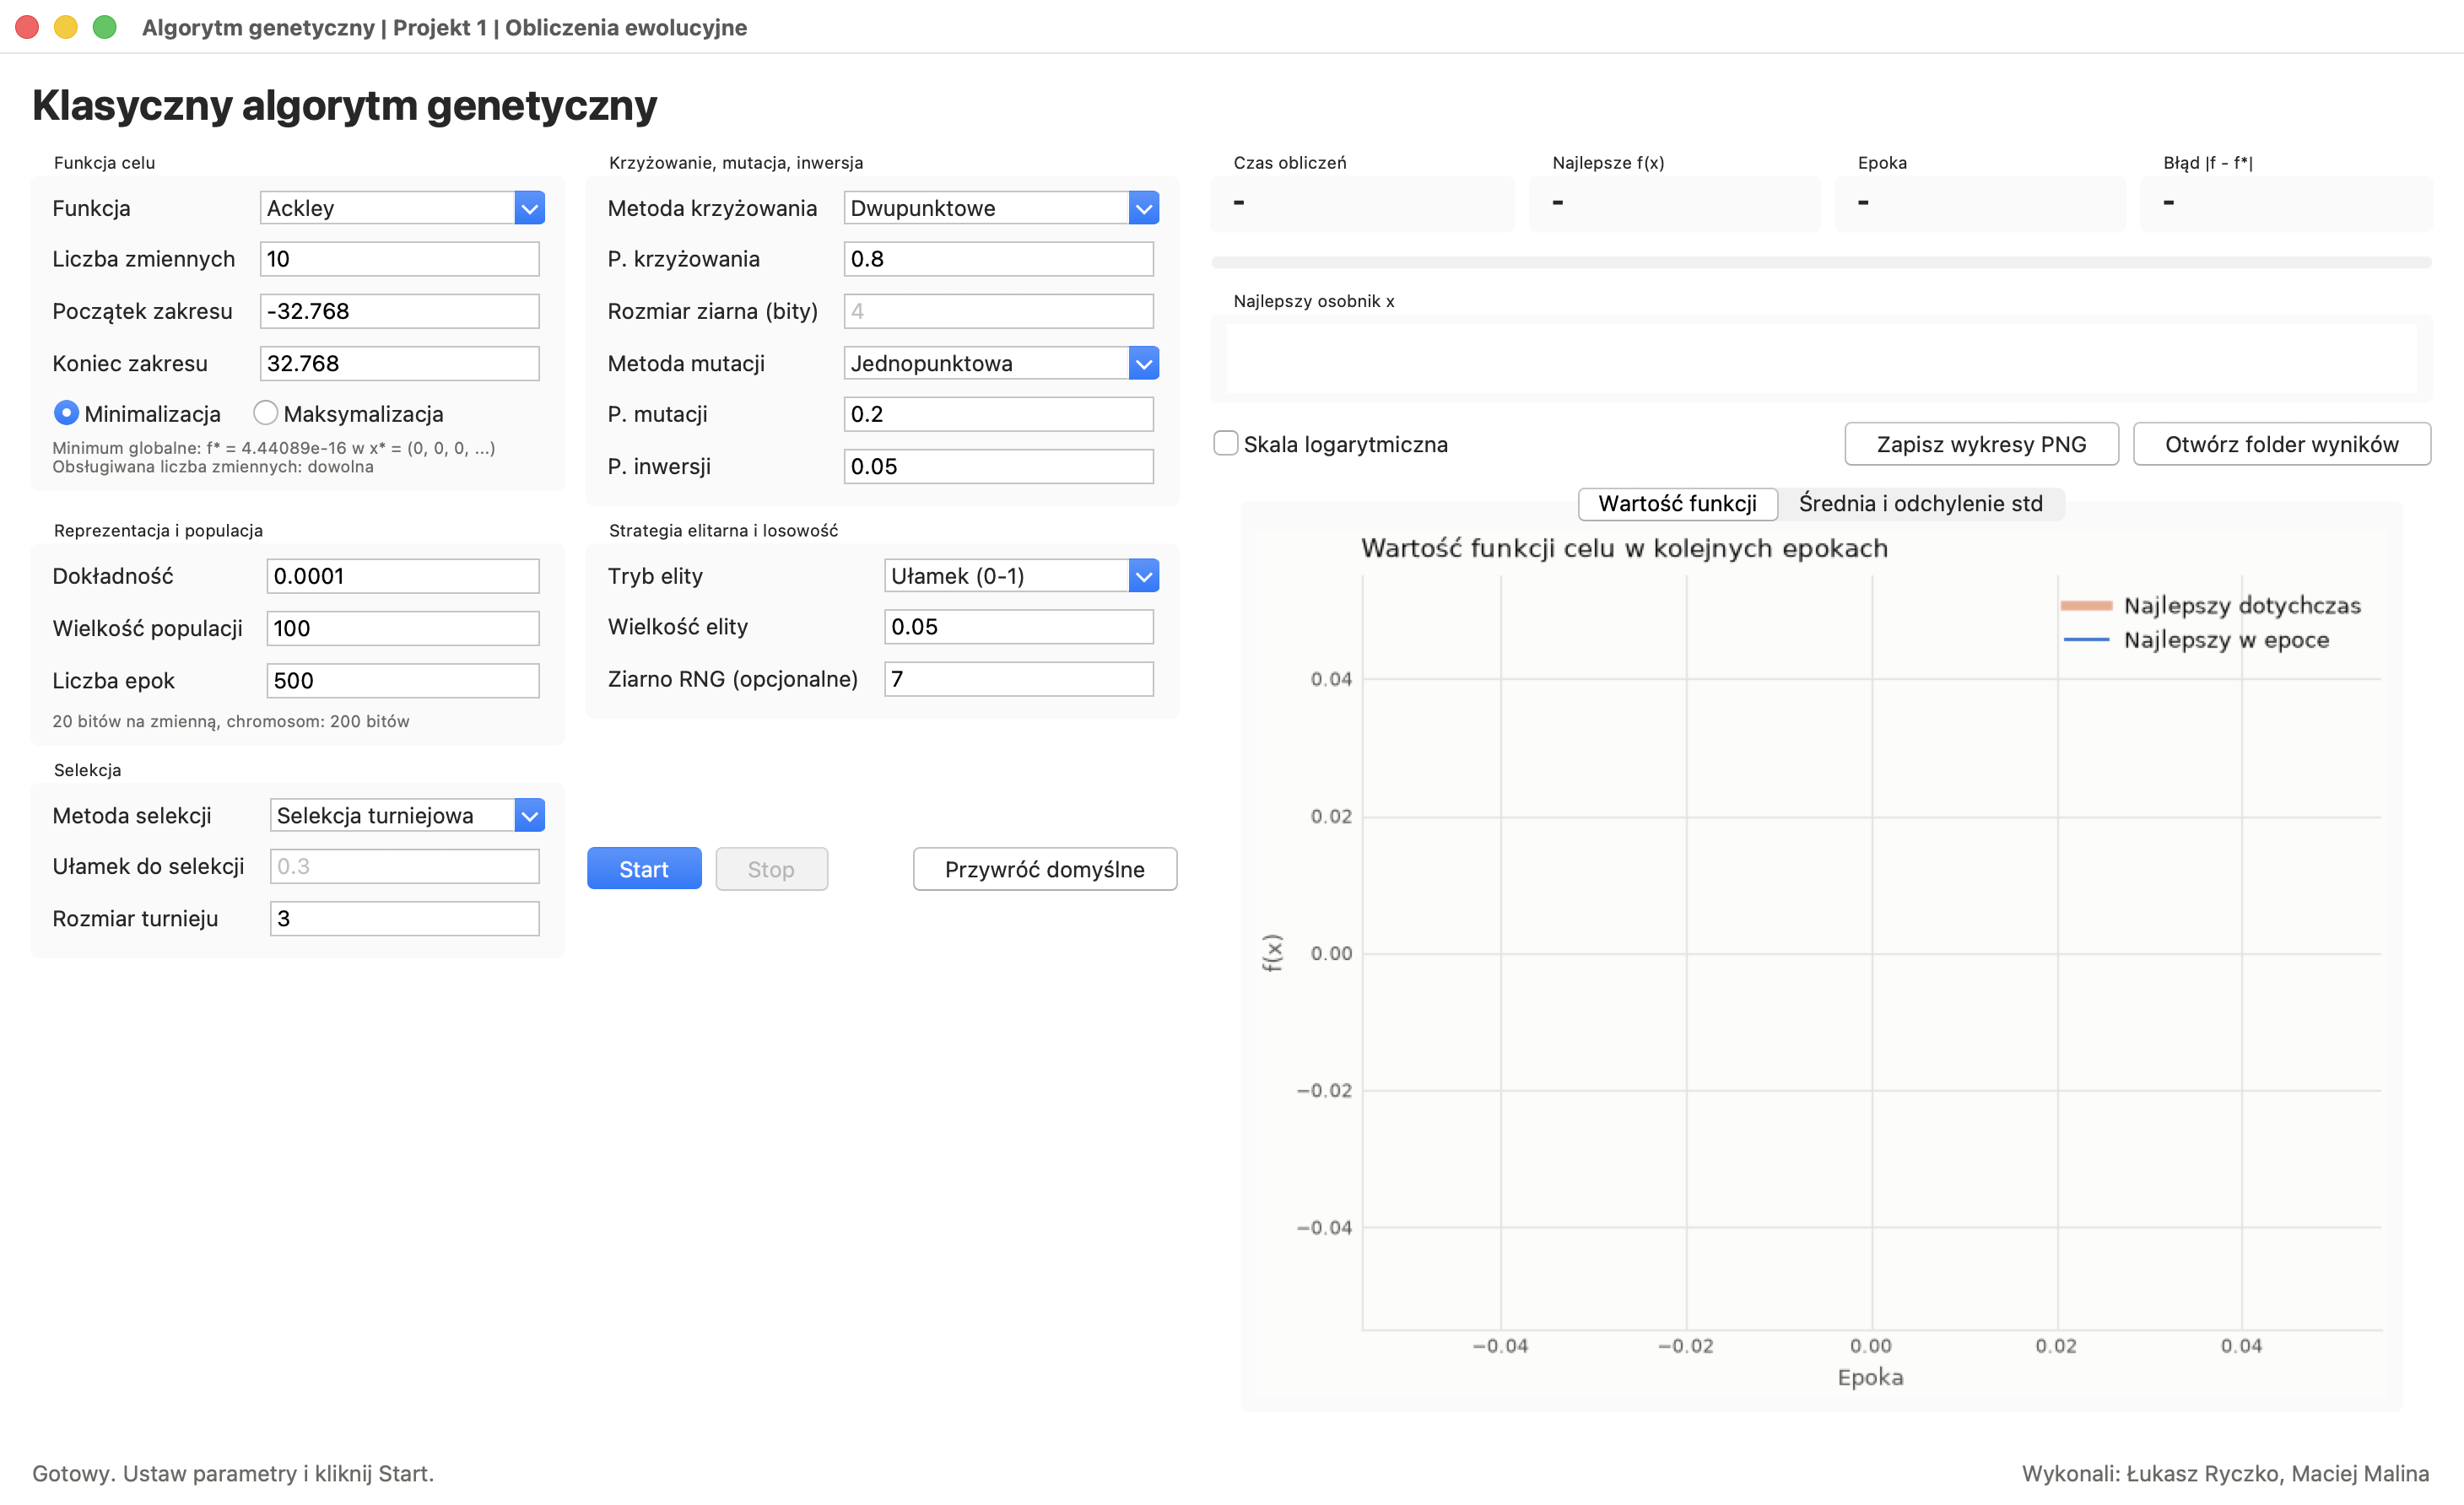
\includegraphics[width=\textwidth]{screens/01_start.png}
  \caption{Aplikacja po uruchomieniu, przed rozpoczęciem obliczeń.}
\end{figure}

\begin{figure}[H]
  \centering
  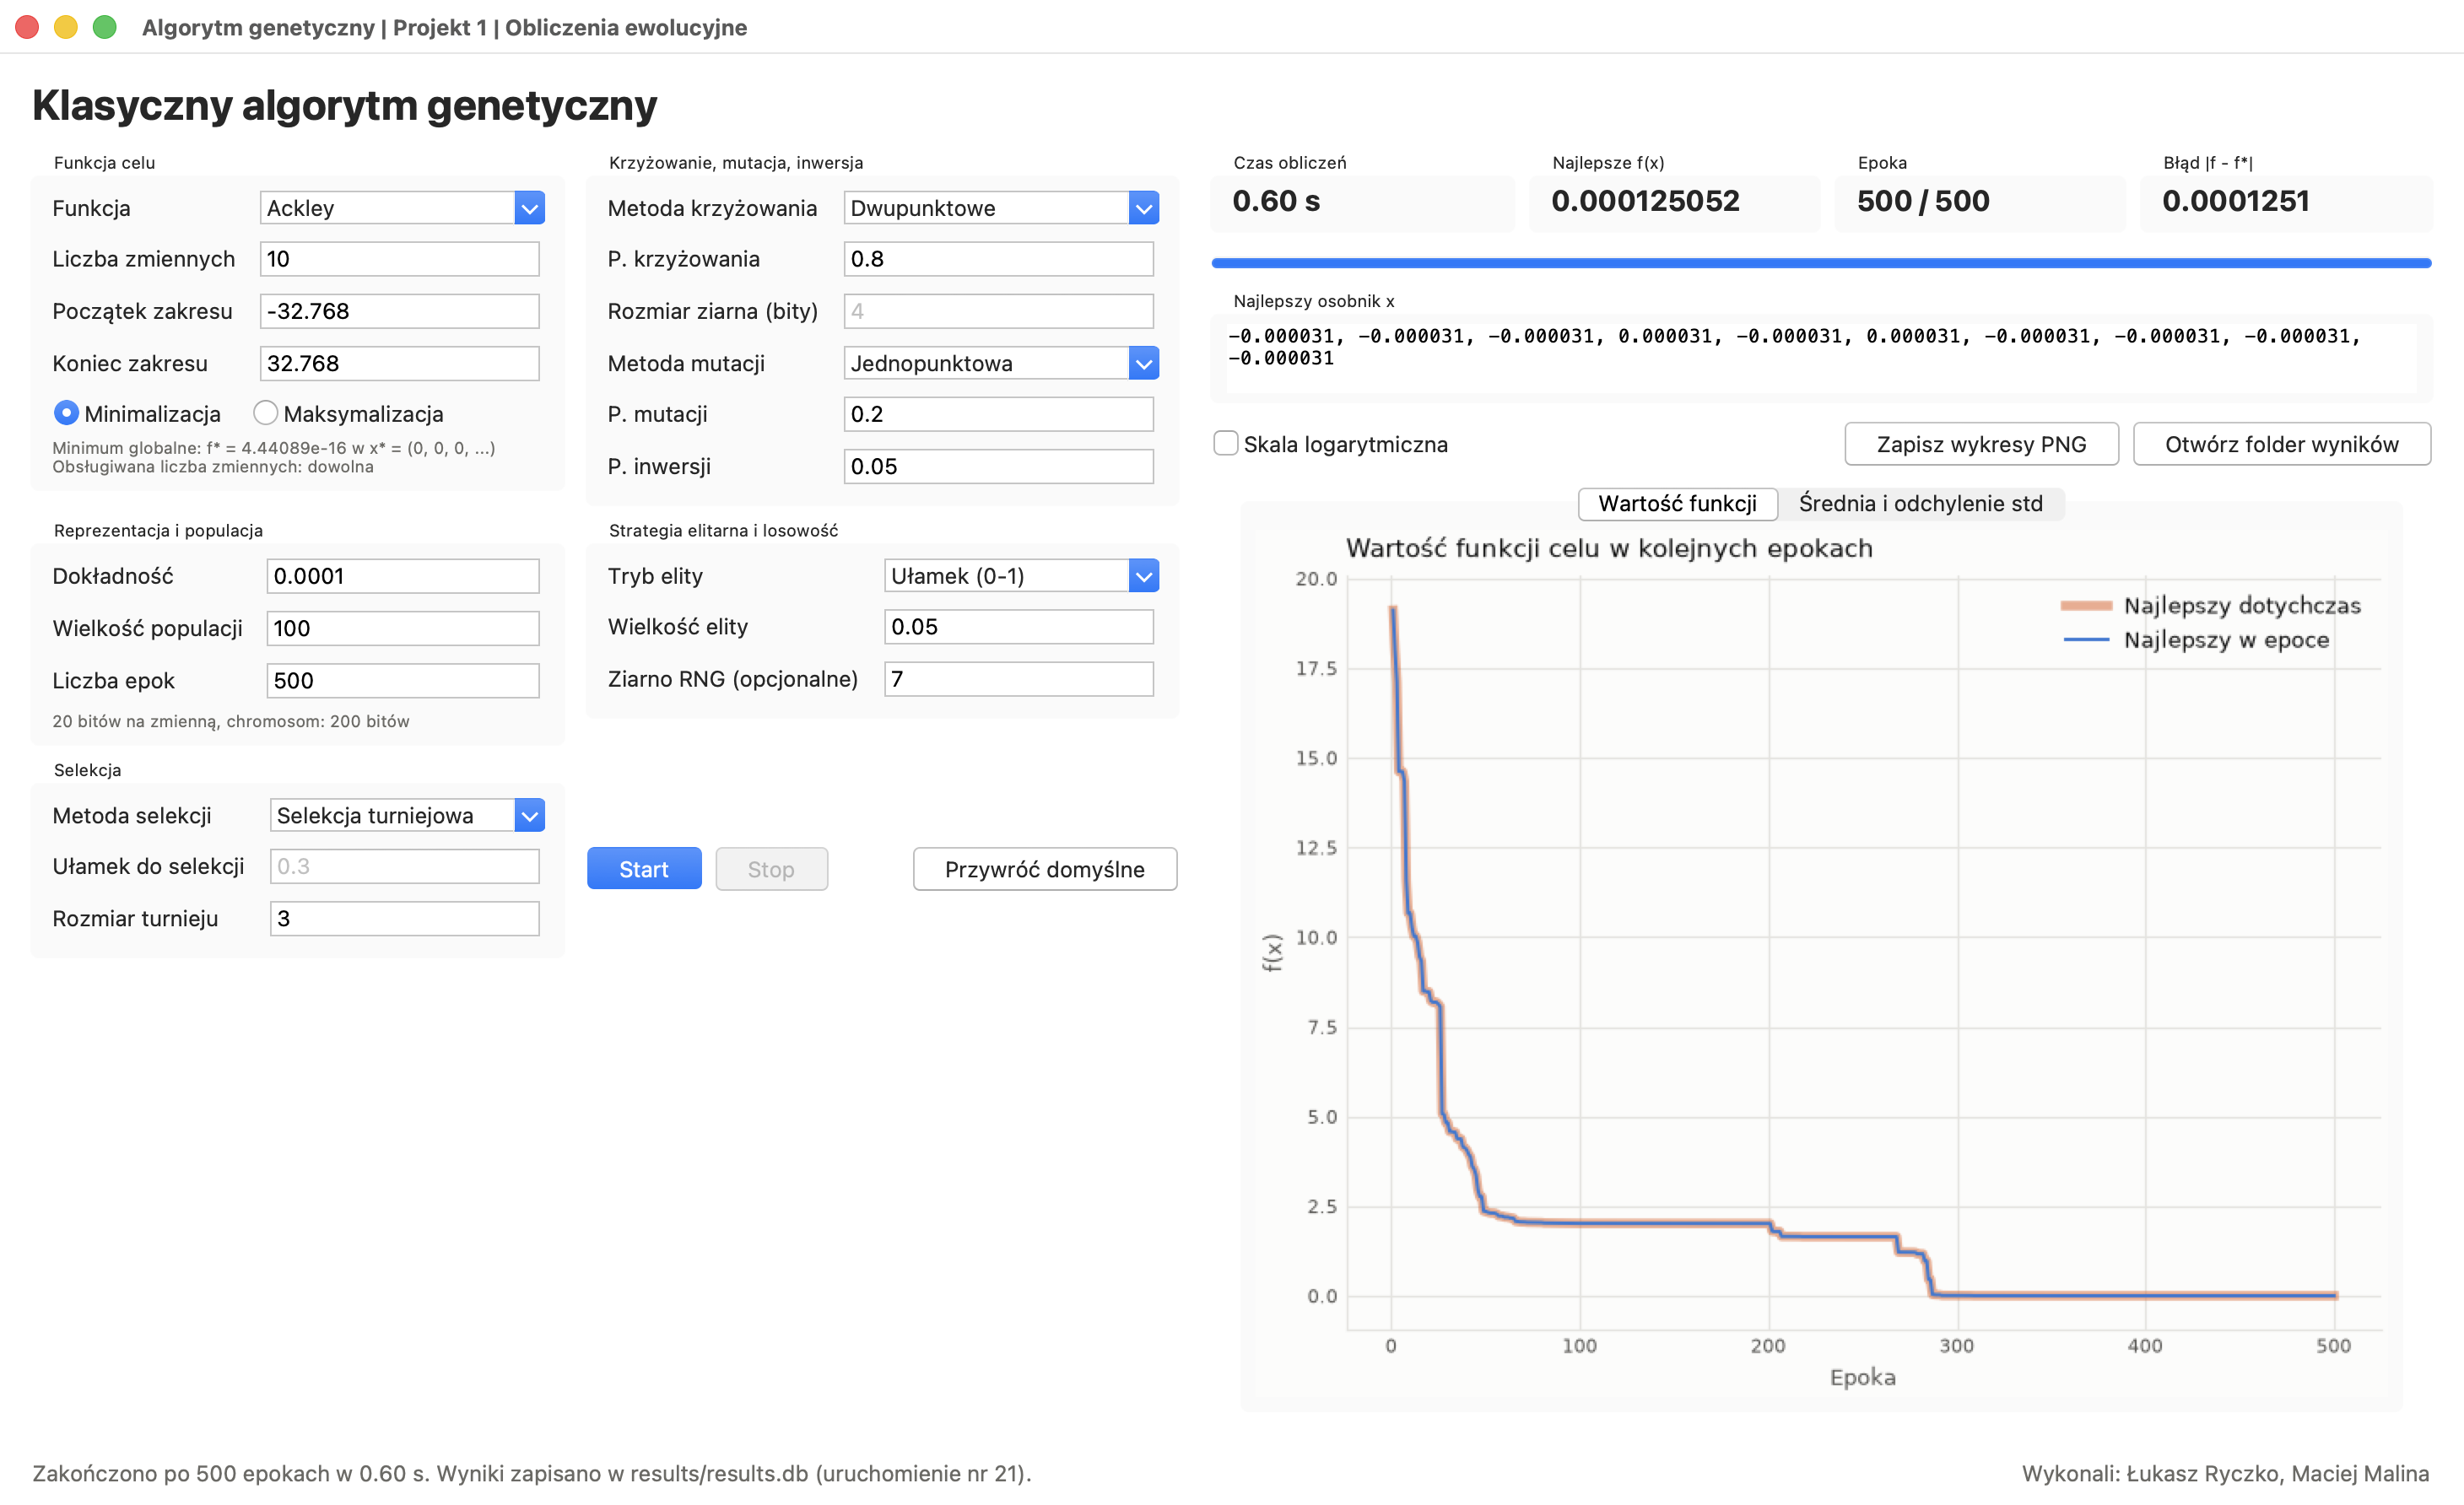
\includegraphics[width=\textwidth]{screens/02_ackley.png}
  \caption{Minimalizacja funkcji Ackley dla 10 zmiennych (selekcja turniejowa, krzyżowanie dwupunktowe).}
\end{figure}

\begin{figure}[H]
  \centering
  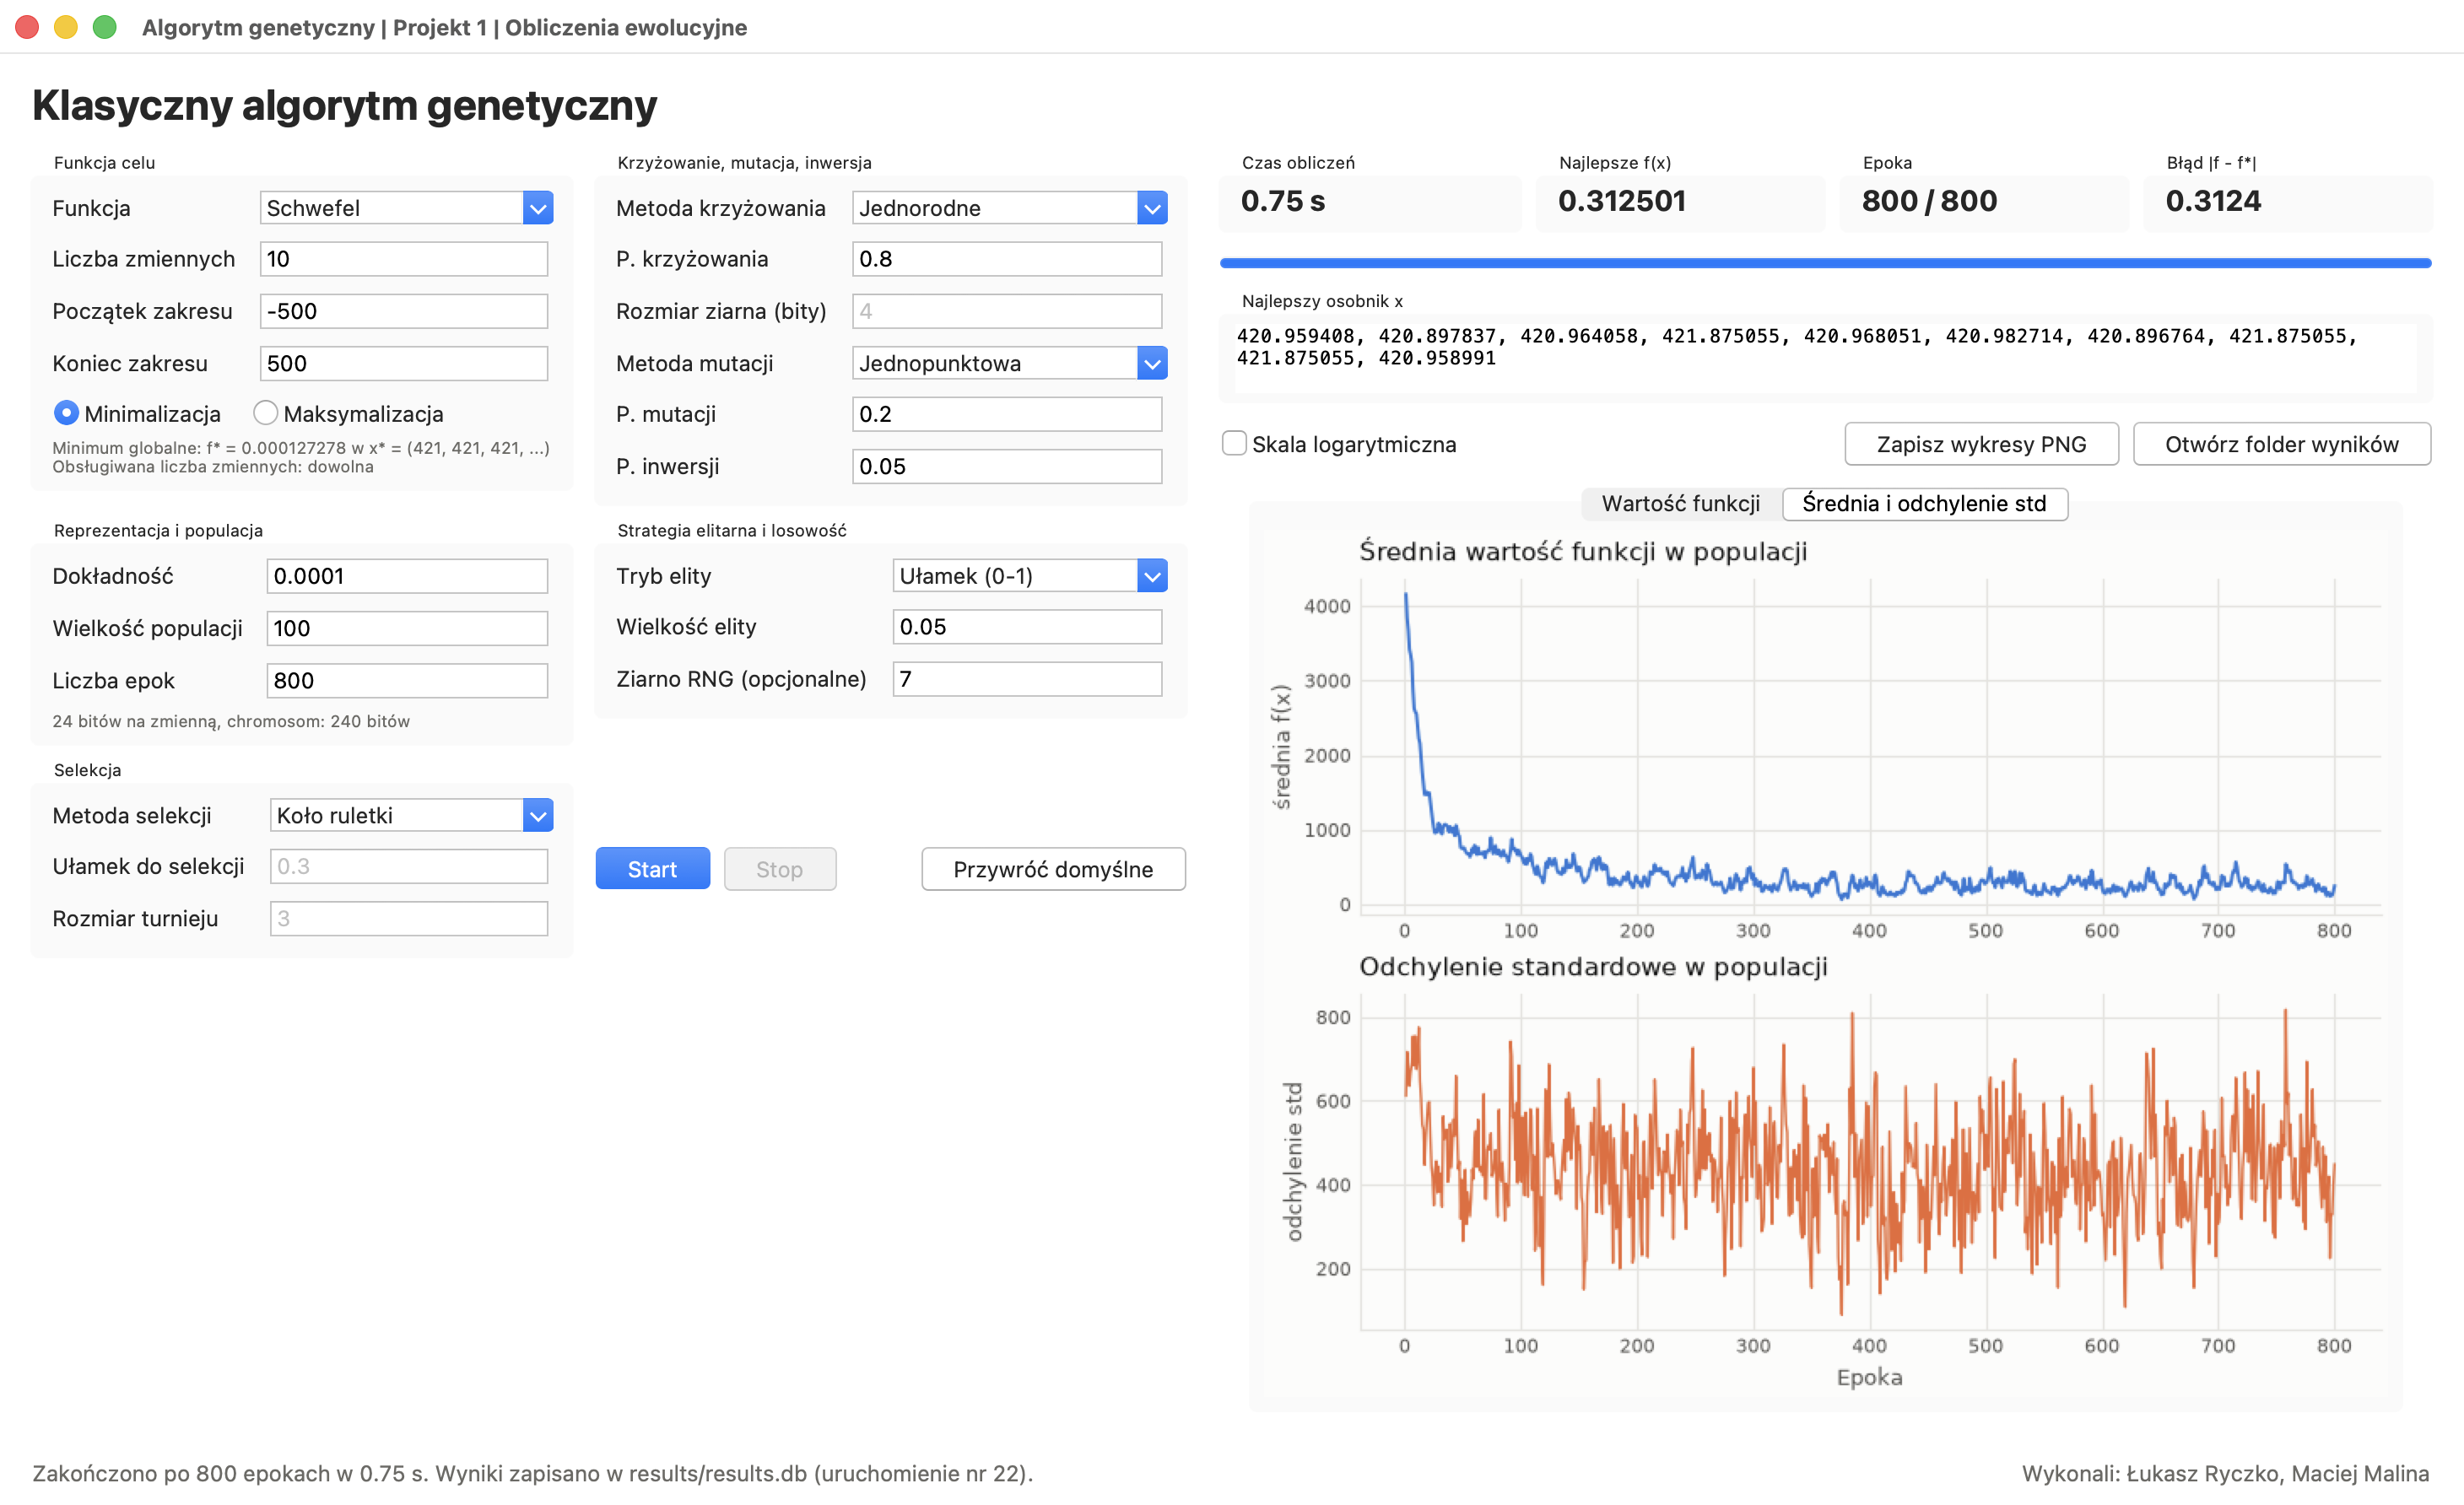
\includegraphics[width=\textwidth]{screens/03_schwefel.png}
  \caption{Funkcja Schwefel, 10 zmiennych: koło ruletki i krzyżowanie jednorodne. Zakładka ze średnią i odchyleniem standardowym.}
\end{figure}

\begin{figure}[H]
  \centering
  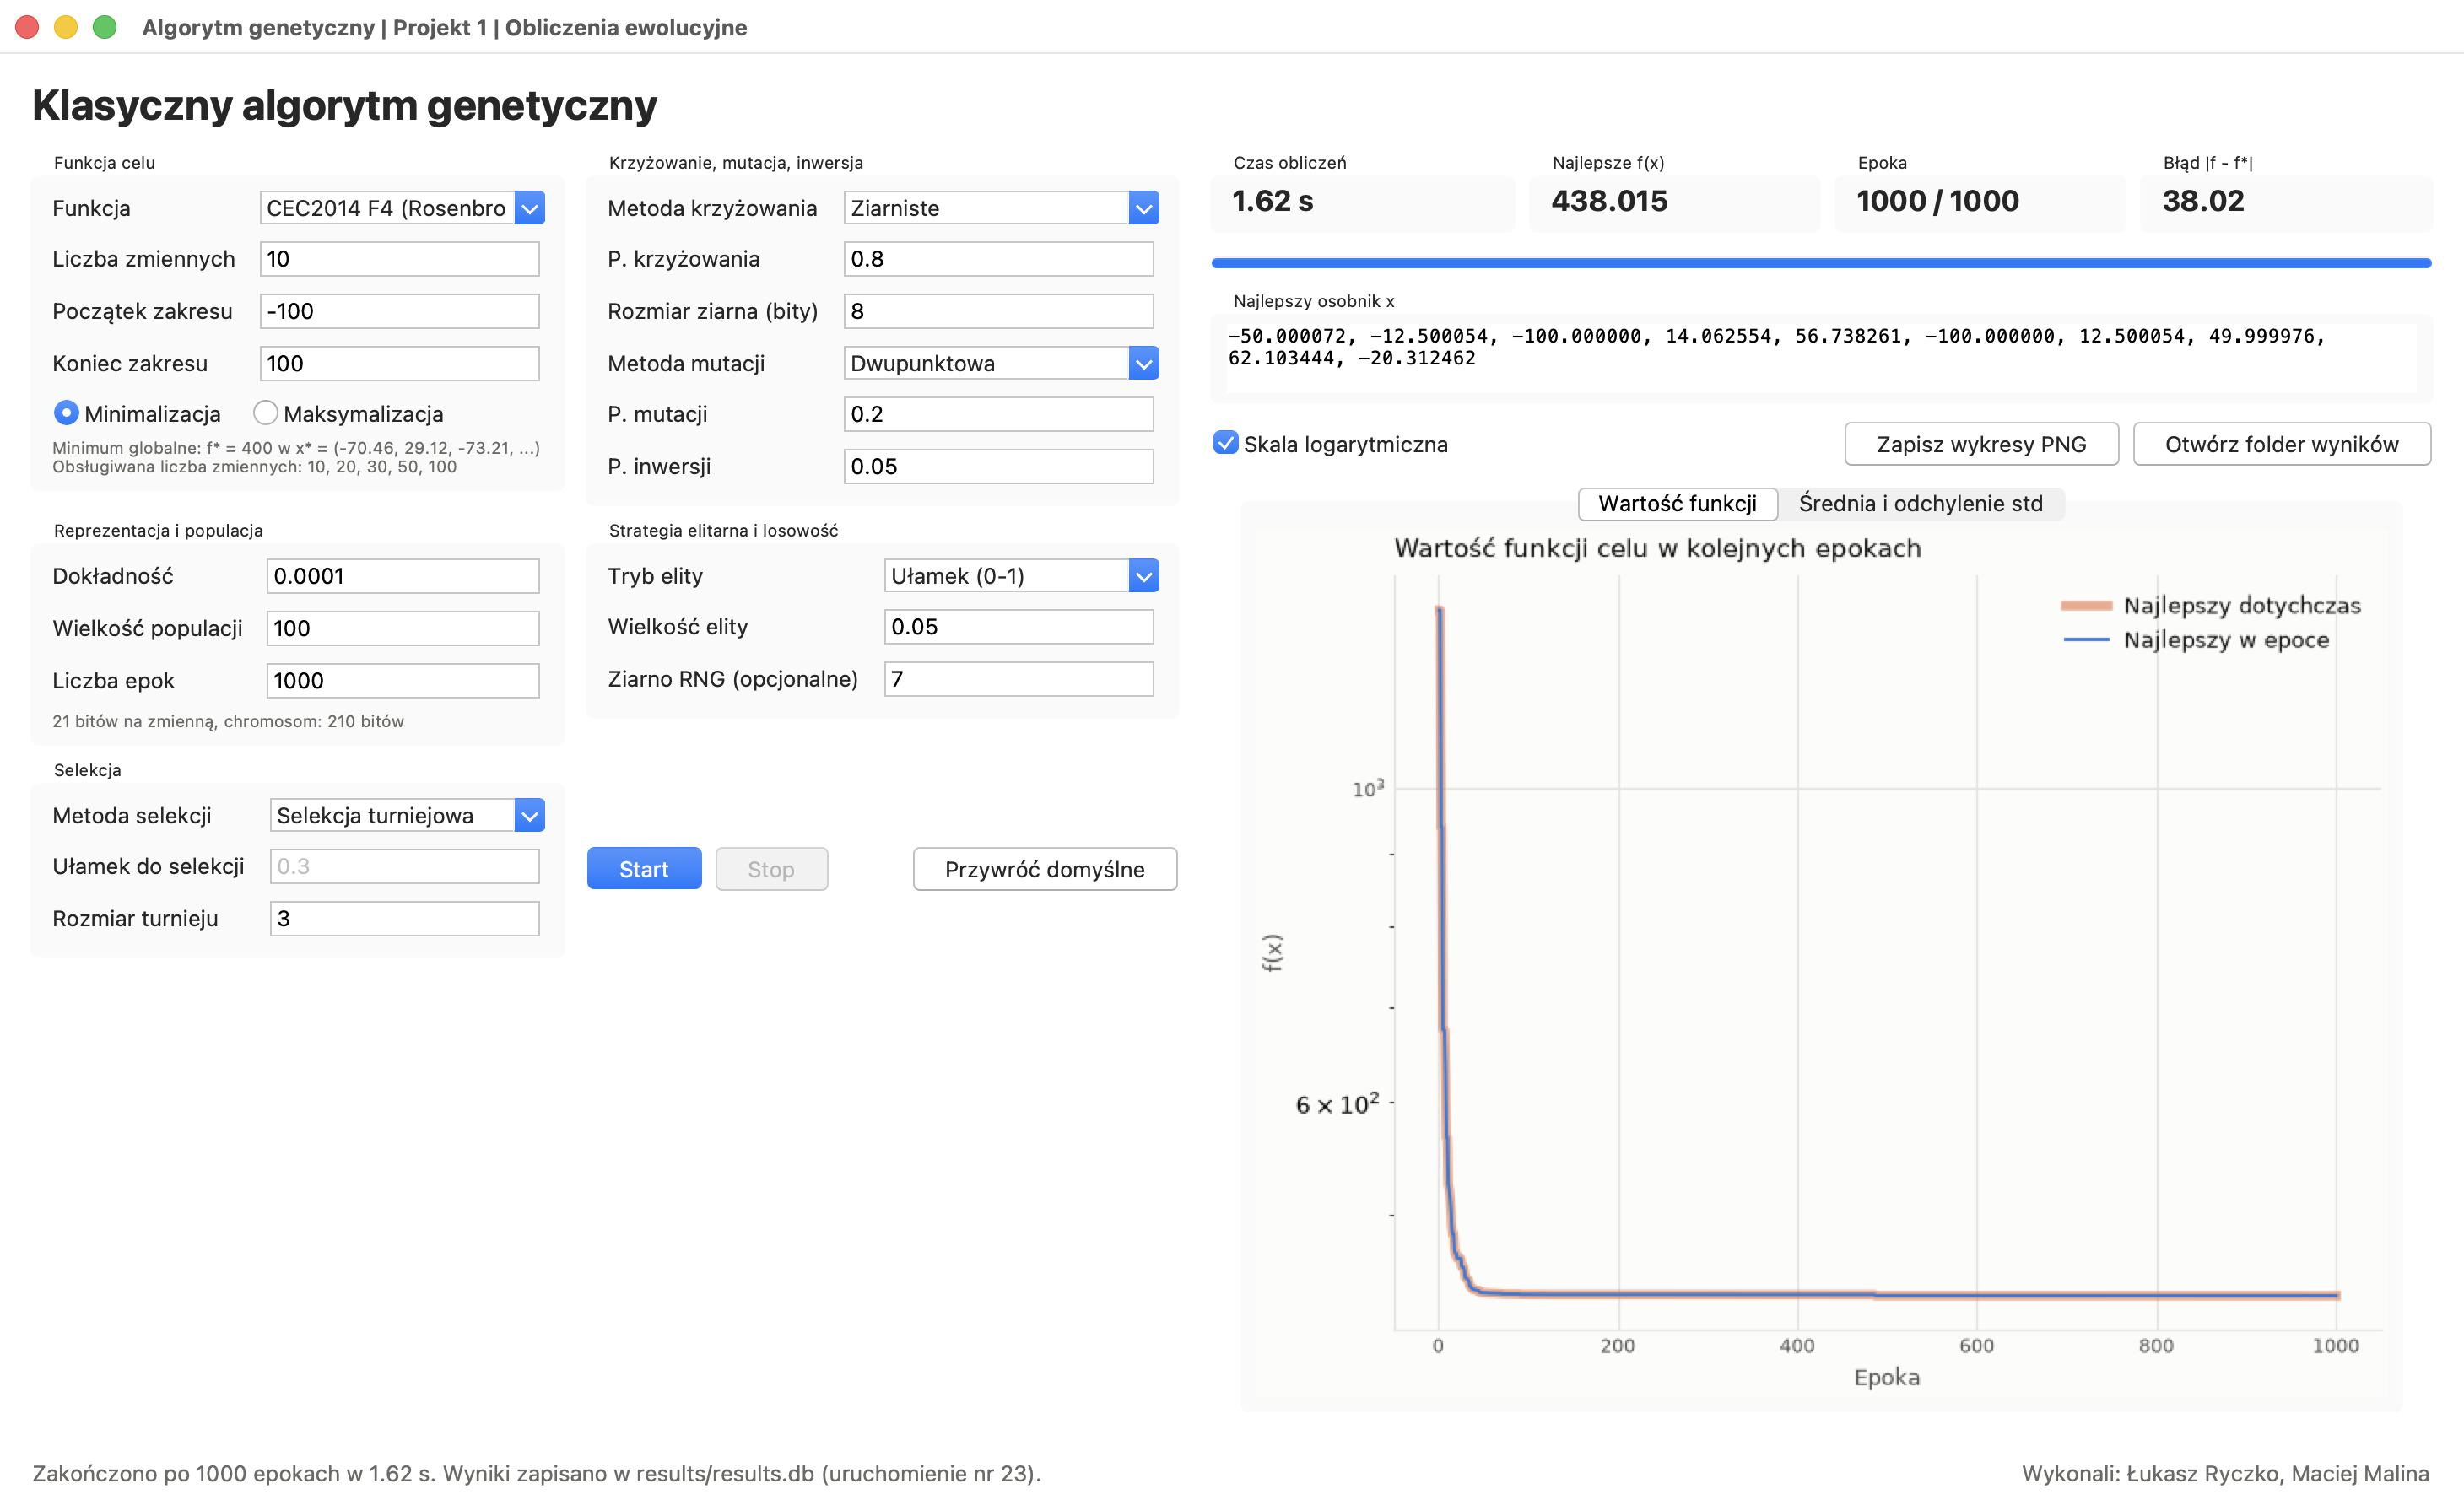
\includegraphics[width=\textwidth]{screens/04_cec_f4.png}
  \caption{CEC2014 F4, 10 zmiennych: krzyżowanie ziarniste, mutacja dwupunktowa, skala logarytmiczna.}
\end{figure}

\begin{figure}[H]
  \centering
  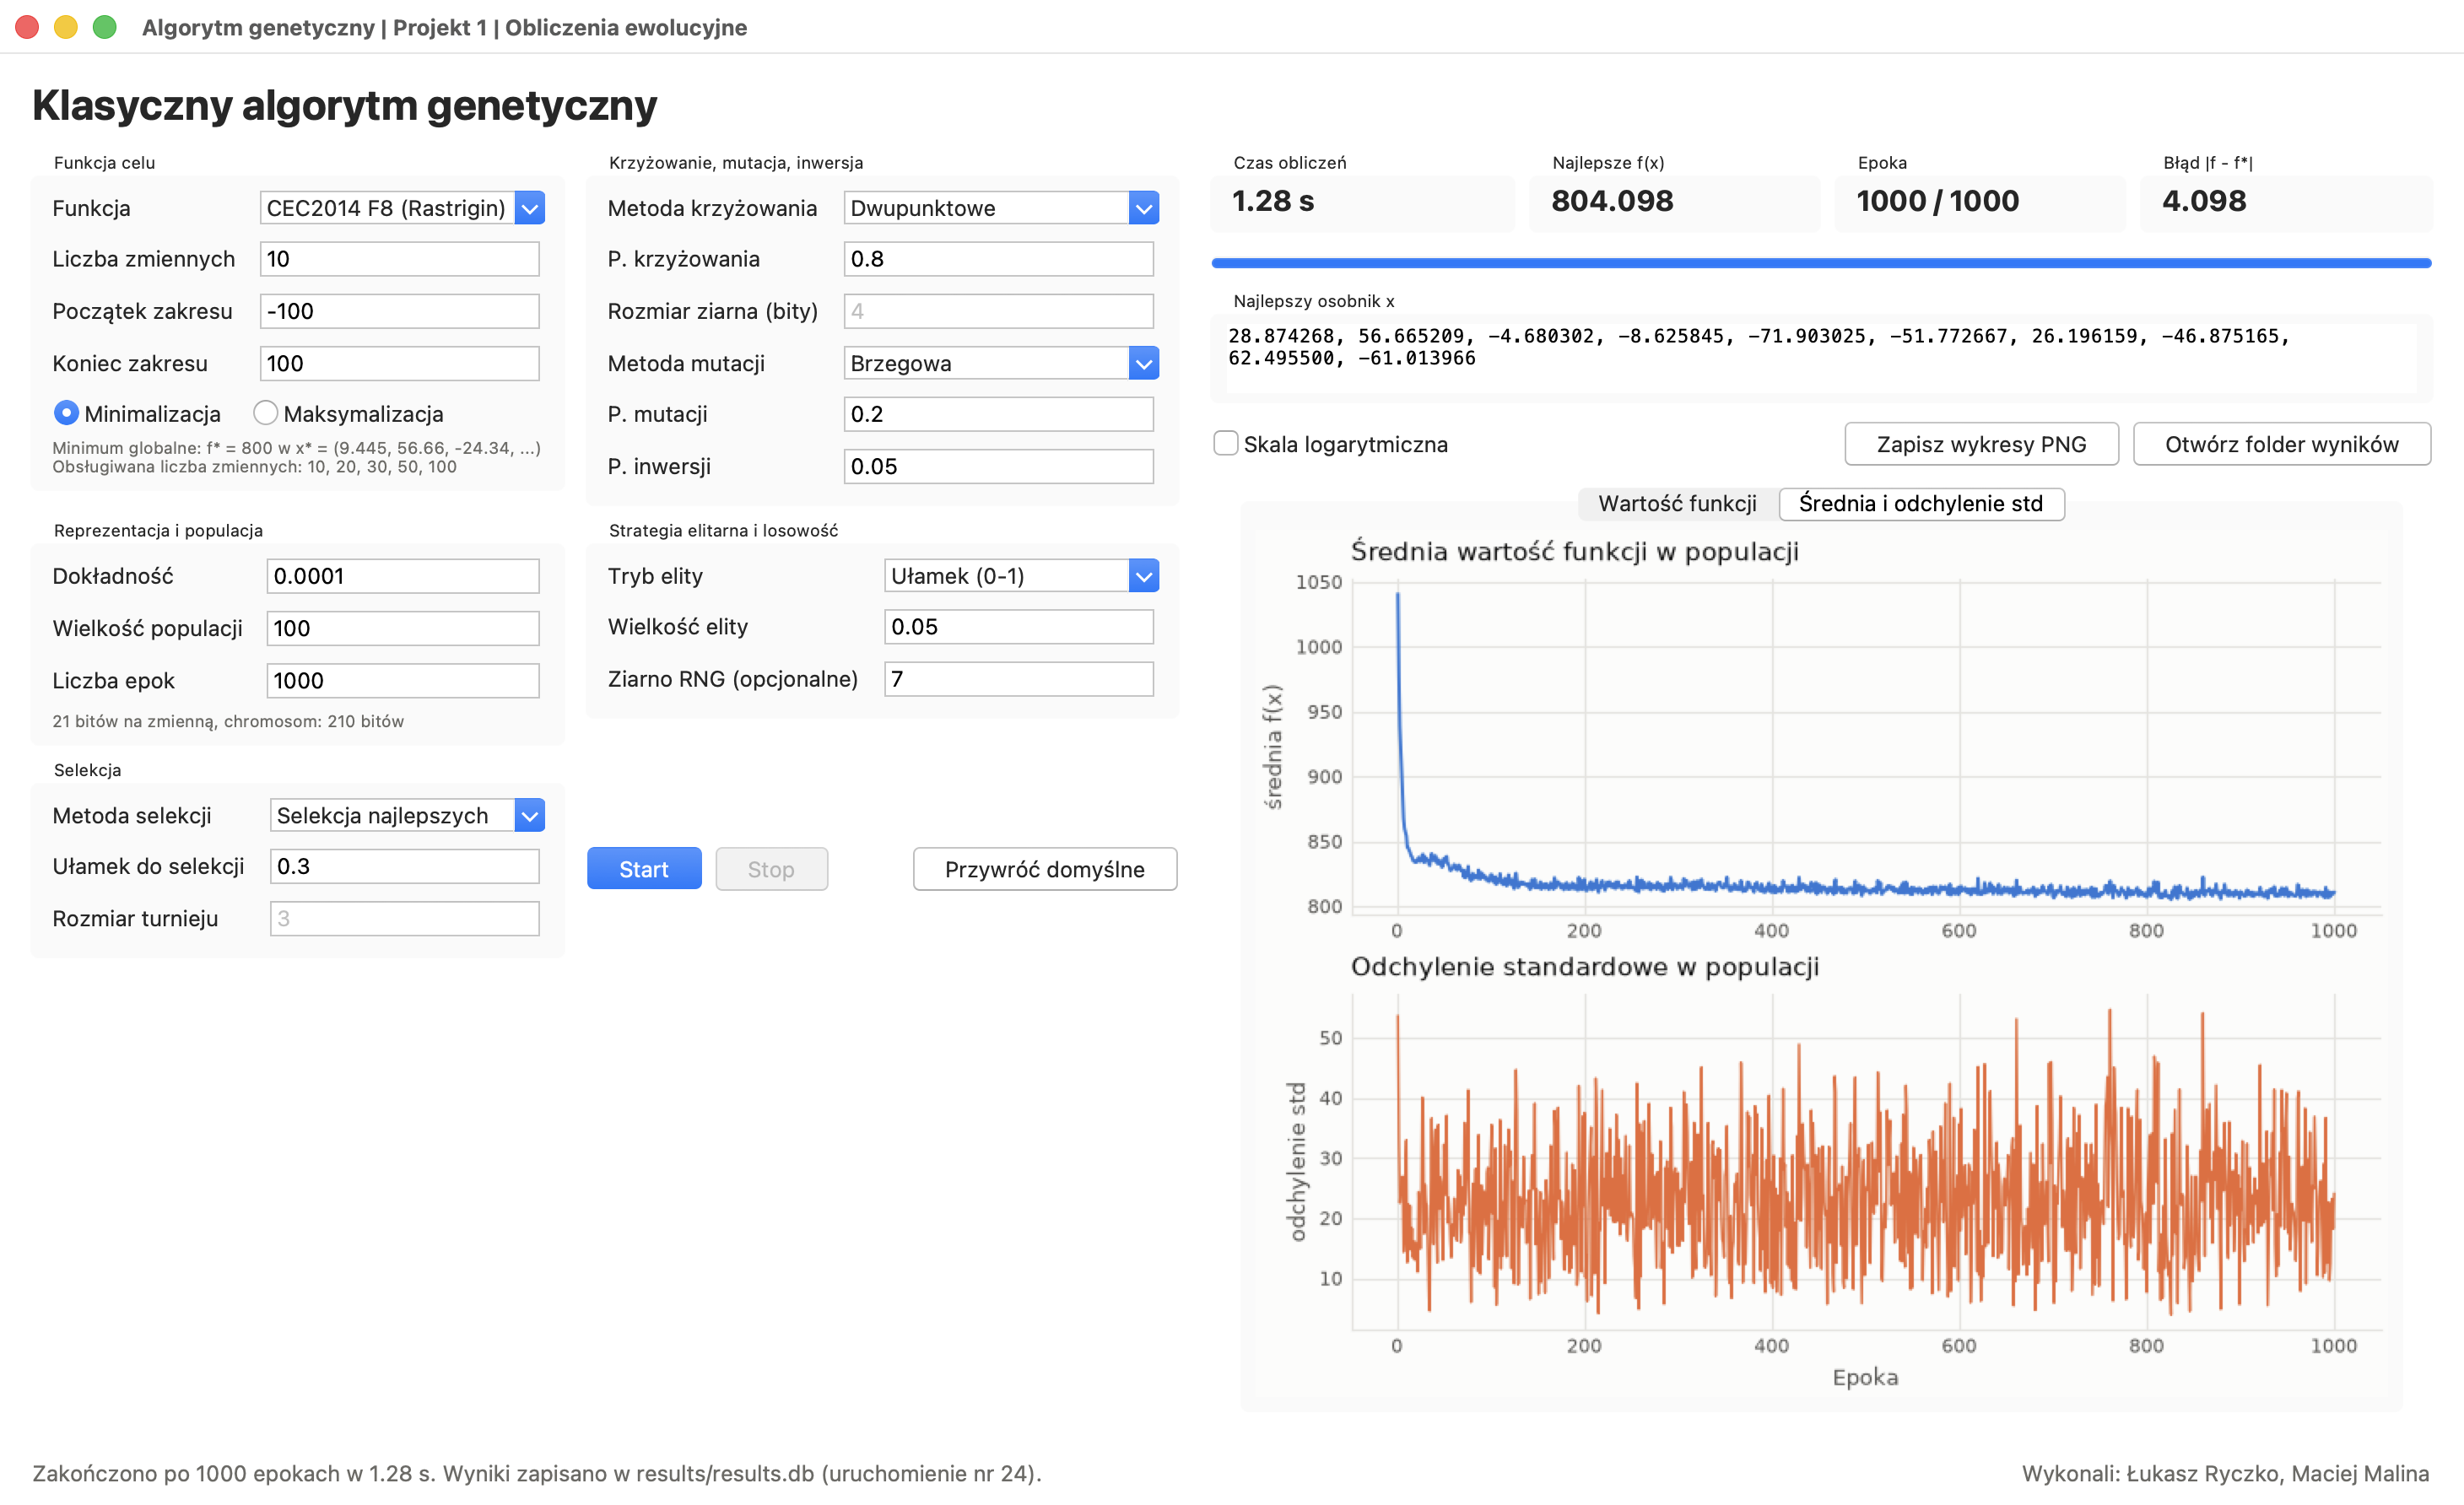
\includegraphics[width=\textwidth]{screens/05_cec_f8.png}
  \caption{CEC2014 F8, 10 zmiennych: selekcja najlepszych, mutacja brzegowa.}
\end{figure}

\begin{figure}[H]
  \centering
  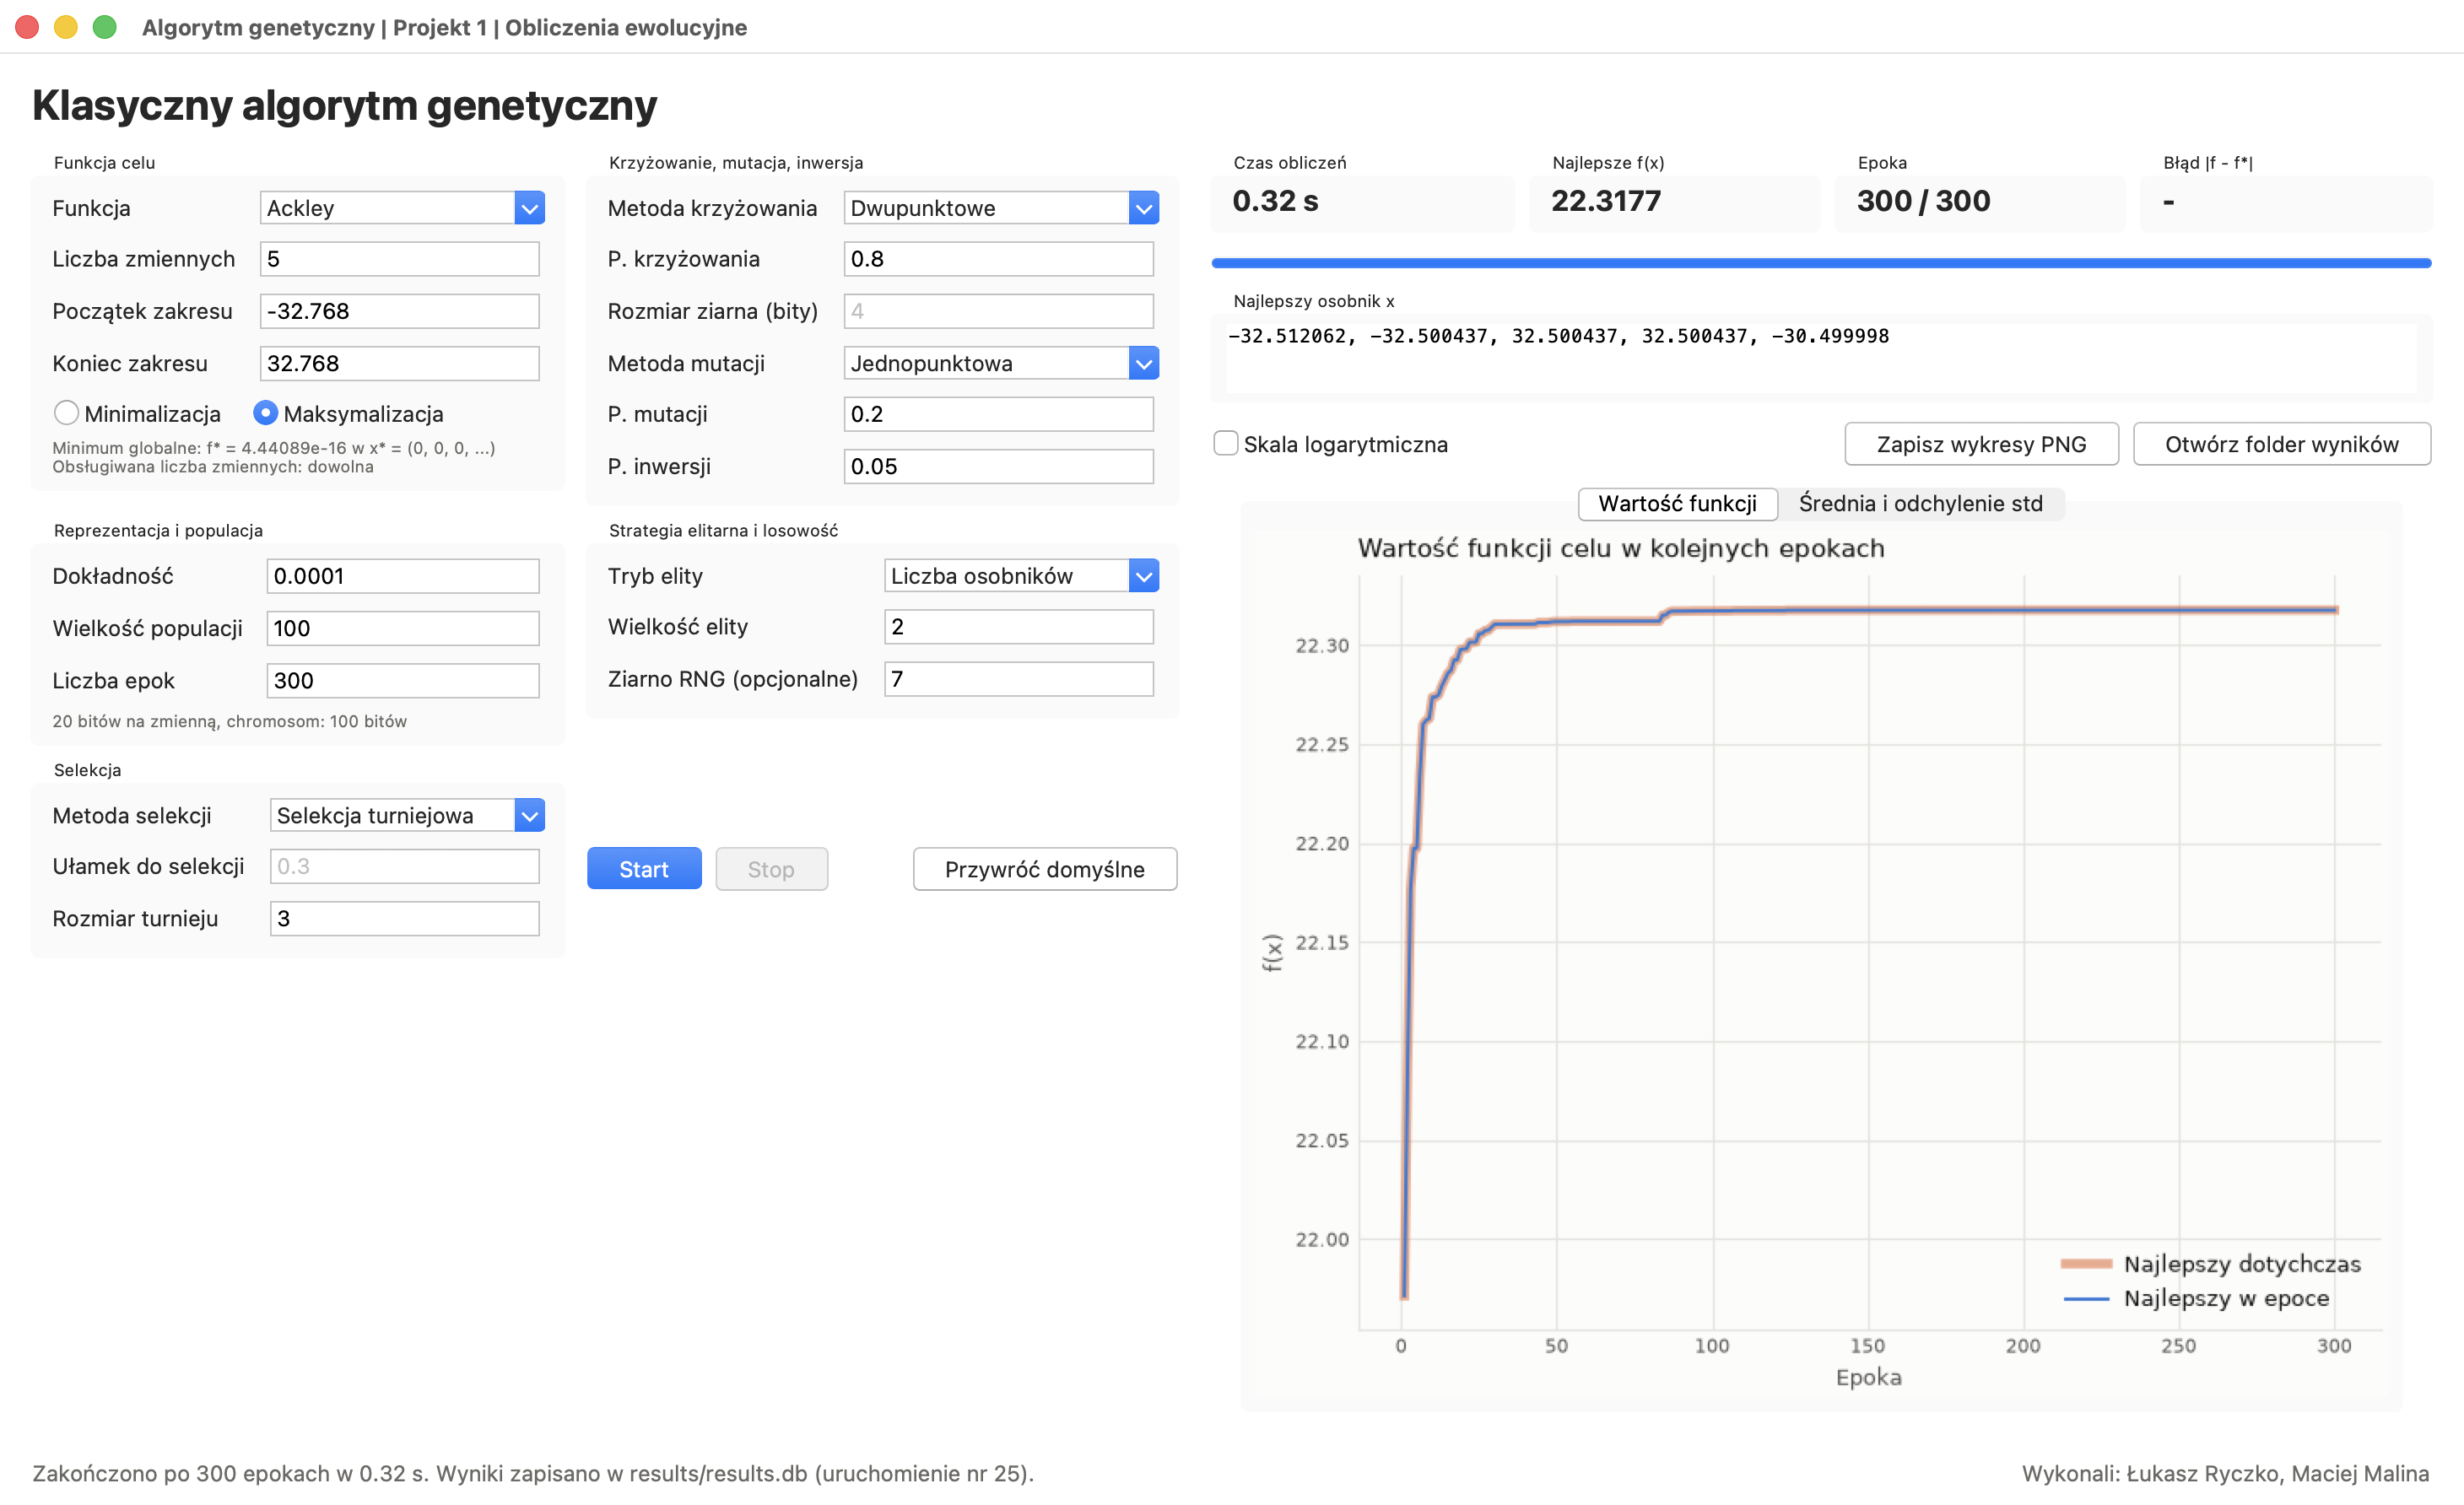
\includegraphics[width=\textwidth]{screens/06_maks.png}
  \caption{Maksymalizacja funkcji Ackley dla 5 zmiennych, elita podana jako liczba osobników (2).
  Algorytm znajduje punkty w pobliżu krawędzi przedziału.}
\end{figure}

\subsection{Zapis wyników}
Każde uruchomienie jest zapisywane w bazie SQLite \texttt{app/results/results.db}, która ma dwie tabele:
\begin{itemize}
  \item \texttt{runs}: jeden wiersz podsumowania na uruchomienie (data, funkcja, liczba zmiennych,
        najlepszy wynik, czas, liczba epok, czy przerwano, najlepszy punkt i pełna konfiguracja w formacie JSON),
  \item \texttt{epochs}: wiersz dla każdej epoki z kolumnami \texttt{run\_id}, \texttt{epoch}, \texttt{best},
        \texttt{mean}, \texttt{std}, \texttt{best\_so\_far}, \texttt{best\_x}
        (klucz obcy \texttt{run\_id} wskazuje wiersz w tabeli \texttt{runs}).
\end{itemize}
Przykładowe zapytanie zwracające przebieg ostatniego uruchomienia:
\begin{lstlisting}[language=SQL]
SELECT epoch, best, mean, std FROM epochs
WHERE run_id = (SELECT MAX(id) FROM runs) ORDER BY epoch;
\end{lstlisting}
Przycisk ,,Zapisz wykresy PNG'' zapisuje oba wykresy do \texttt{app/results/plots/}.

\section{Wybrane funkcje testowe}

Wybraliśmy dwie proste funkcje z biblioteki benchmark\_functions (Ackley i Schwefel) oraz dwie
funkcje z zestawu CEC 2014 z biblioteki opfunu (F4 i F8). Wszystkie pozwalają ustawić różną liczbę
zmiennych (funkcje CEC 2014 tylko 10, 20, 30, 50 lub 100).

Początkowo rozważaliśmy funkcję CEC2014 F10 (Shifted Schwefel). Okazało się jednak, że jej
implementacja w opfunu 1.0.1 ma błąd znaku w obsłudze punktów spoza przedziału $[-500, 500]$:
algorytm znajdował wartości około $-3000$, czyli mniejsze od optimum równego 1000. Z tego powodu
wybraliśmy funkcję F8.

\subsection{Ackley}
\[
  f(x) = -20\exp\!\left(-0.2\sqrt{\tfrac{1}{n}\textstyle\sum_{i=1}^{n} x_i^2}\right)
         - \exp\!\left(\tfrac{1}{n}\textstyle\sum_{i=1}^{n}\cos(2\pi x_i)\right) + 20 + e,
  \qquad x_i \in [-32.768,\ 32.768].
\]
Minimum globalne $f(x^*) = 0$ w punkcie $x^* = (0, \ldots, 0)$. Funkcja ma bardzo wiele minimów
lokalnych, ale wyraźne globalne ,,lejkowate'' minimum.

\begin{figure}[H]
  \centering
  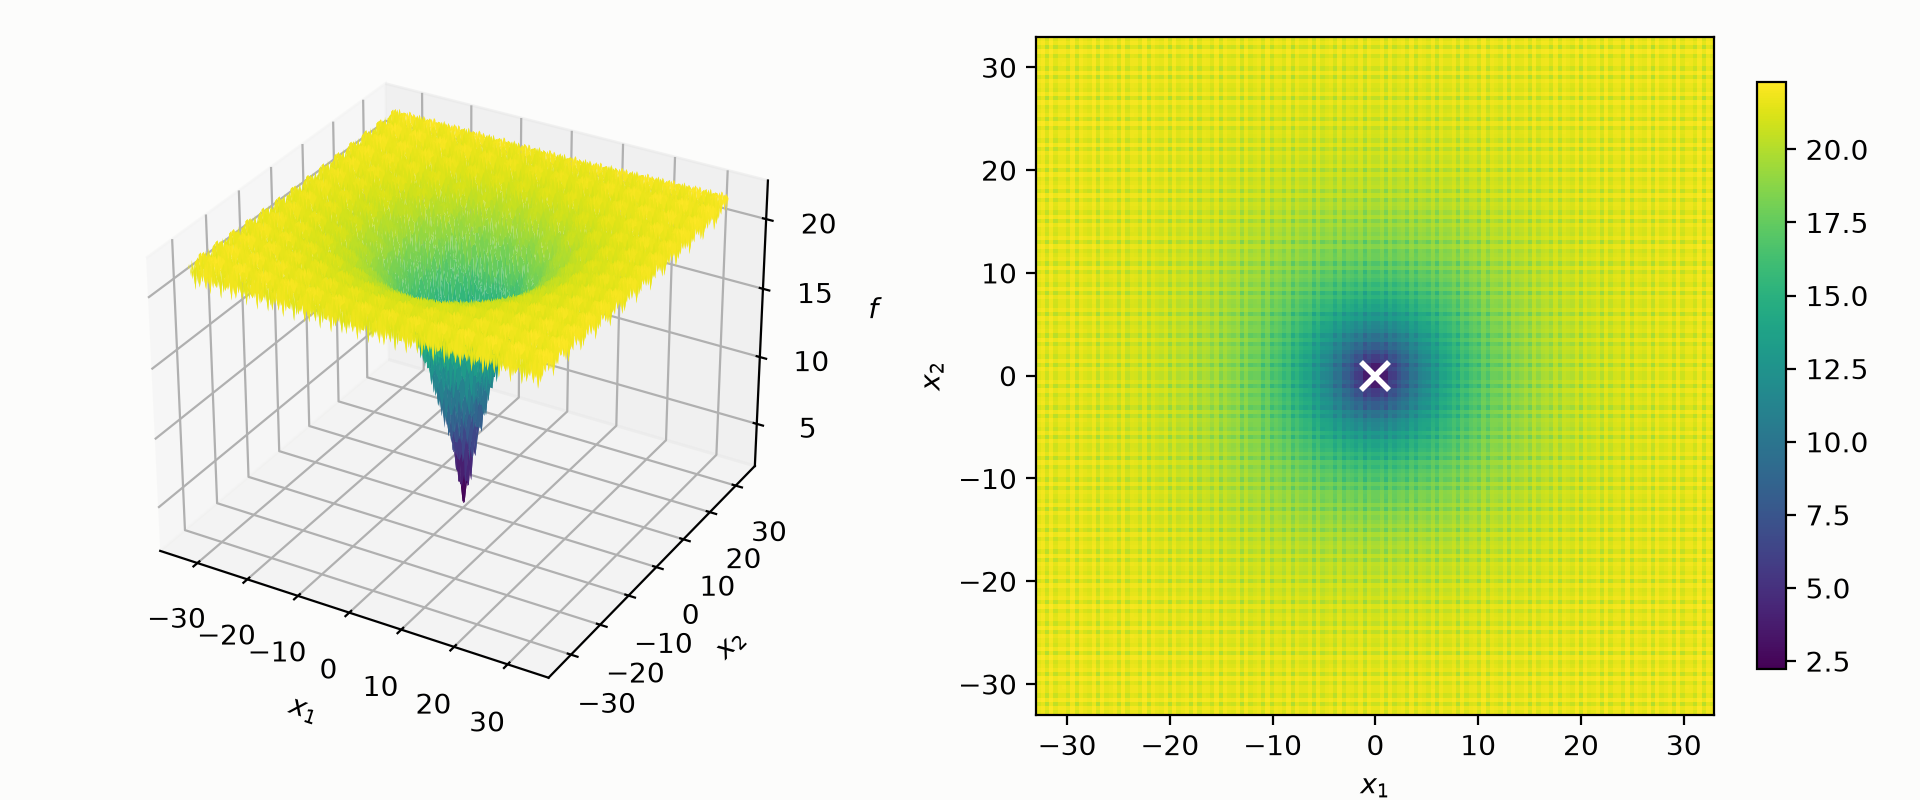
\includegraphics[width=0.92\textwidth]{function_ackley.png}
  \caption{Funkcja Ackley dla 2 zmiennych: wykres 3D i mapa ciepła (krzyżyk oznacza optimum).}
\end{figure}

\subsection{Schwefel}
\[
  f(x) = 418.9829\, n - \sum_{i=1}^{n} x_i \sin\!\left(\sqrt{|x_i|}\right),
  \qquad x_i \in [-500,\ 500].
\]
Minimum globalne $f(x^*) \approx 0$ w punkcie $x^* = (420.9687, \ldots, 420.9687)$. Najlepsze
minimum lokalne leży daleko od globalnego, przy przeciwnym końcu przedziału, co utrudnia optymalizację.

\begin{figure}[H]
  \centering
  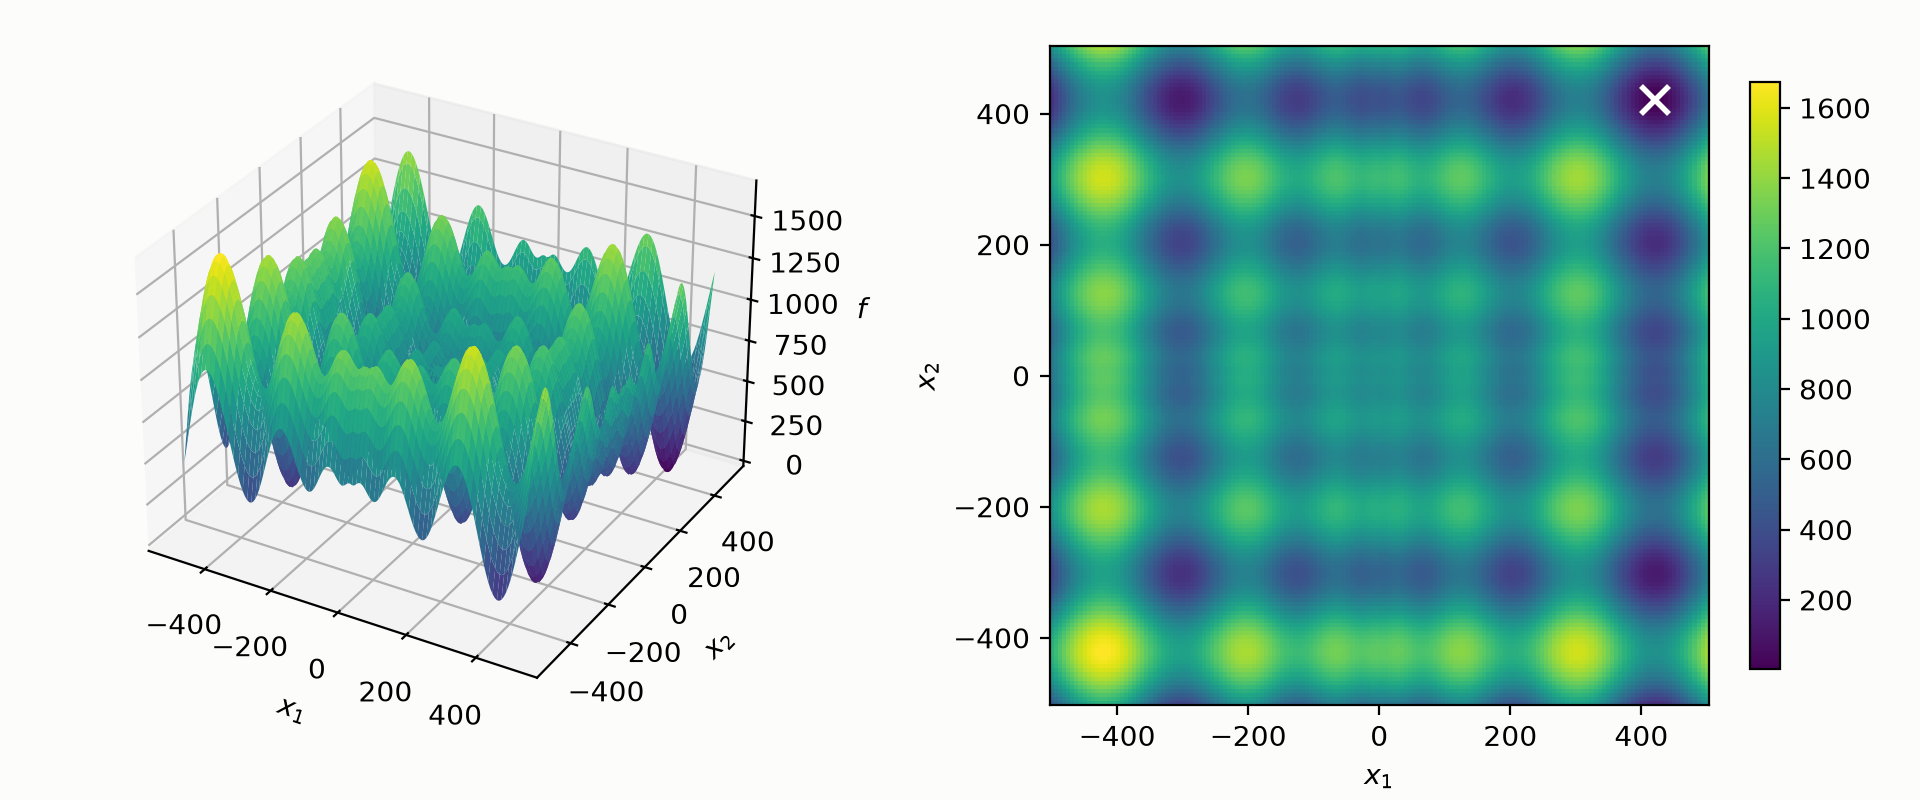
\includegraphics[width=0.92\textwidth]{function_schwefel.png}
  \caption{Funkcja Schwefel dla 2 zmiennych.}
\end{figure}

\subsection{CEC2014 F4: Shifted and Rotated Rosenbrock's Function}
\[
  F_4(x) = f_4\!\left(\mathbf{M}_4\left(\tfrac{2.048\,(x-o_4)}{100}\right) + 1\right) + 400,
  \qquad
  f_4(z) = \sum_{i=1}^{D-1}\left(100\,(z_i^2 - z_{i+1})^2 + (z_i - 1)^2\right),
\]
gdzie $o_4$ to wektor przesunięcia, a $\mathbf{M}_4$ macierz obrotu. Przedział $[-100, 100]^D$,
minimum $F_4(x^*) = 400$ w punkcie $x^* = o_4$. Obrót powoduje, że zmienne są ze sobą powiązane,
a dno ,,doliny'' Rosenbrocka jest bardzo płaskie.

\begin{figure}[H]
  \centering
  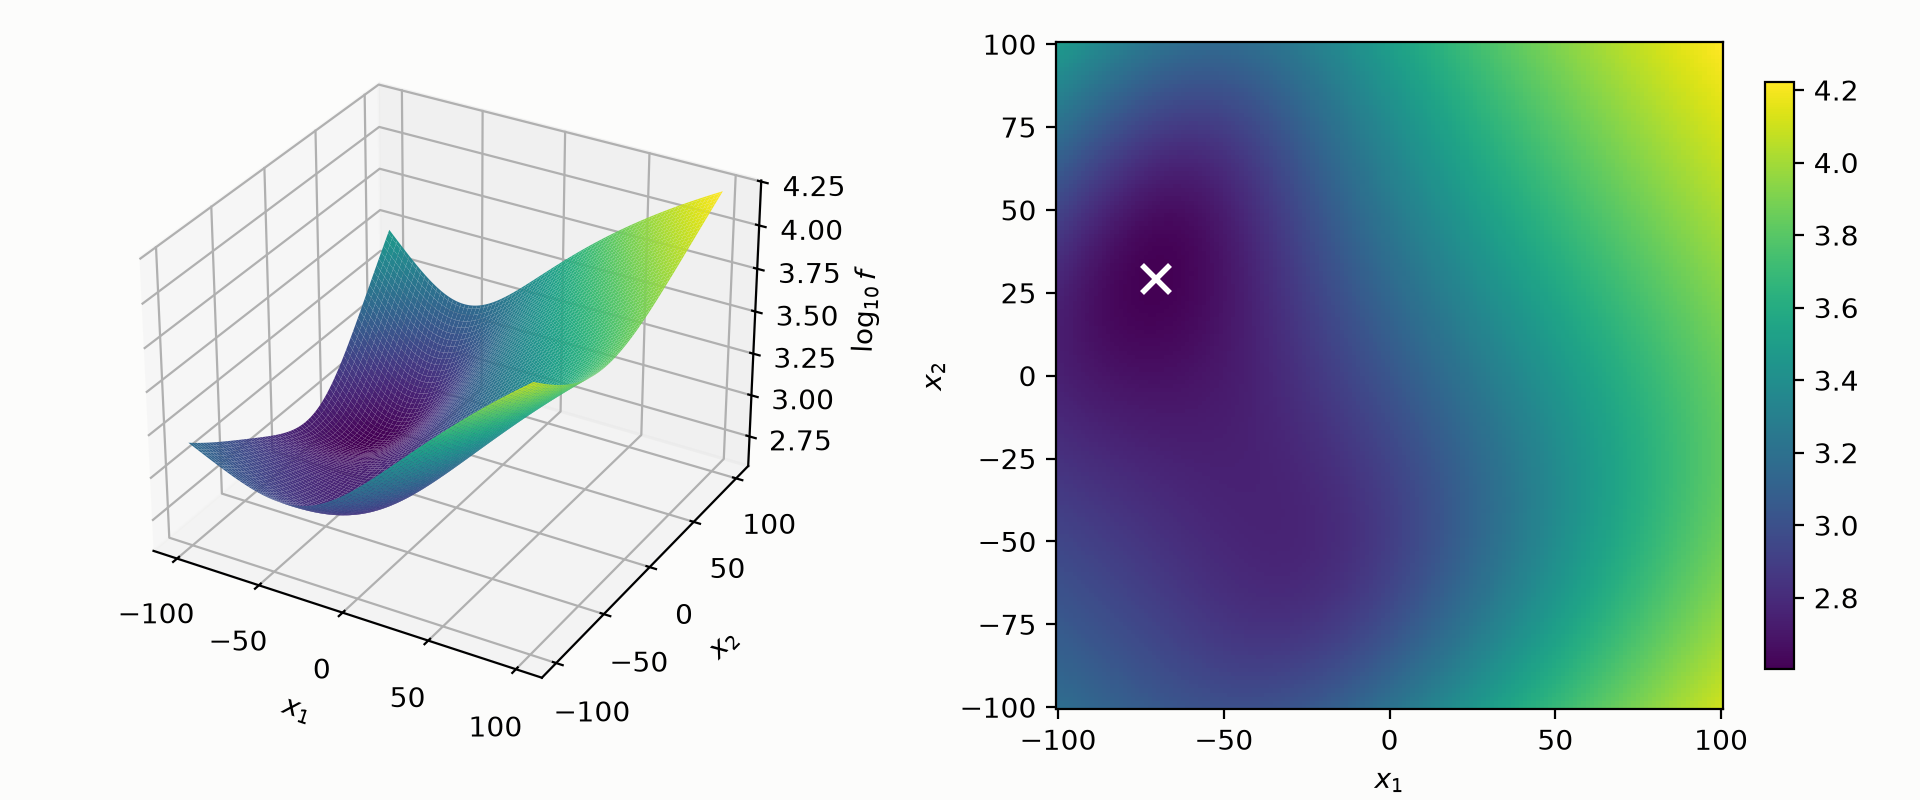
\includegraphics[width=0.92\textwidth]{function_cec2014_f4.png}
  \caption{CEC2014 F4: przekrój funkcji 10 zmiennych przez optimum w płaszczyźnie $(x_1, x_2)$,
  pozostałe zmienne ustalone na wartościach optymalnych. Oś pionowa w skali $\log_{10}$.}
\end{figure}

\subsection{CEC2014 F8: Shifted Rastrigin's Function}
\[
  F_8(x) = f_8\!\left(\tfrac{5.12\,(x-o_8)}{100}\right) + 800,
  \qquad
  f_8(z) = \sum_{i=1}^{D}\left(z_i^2 - 10\cos(2\pi z_i) + 10\right).
\]
Przedział $[-100, 100]^D$, minimum $F_8(x^*) = 800$ w punkcie $x^* = o_8$. Funkcja jest separowalna,
ale ma ogromną liczbę regularnie rozłożonych minimów lokalnych.

\begin{figure}[H]
  \centering
  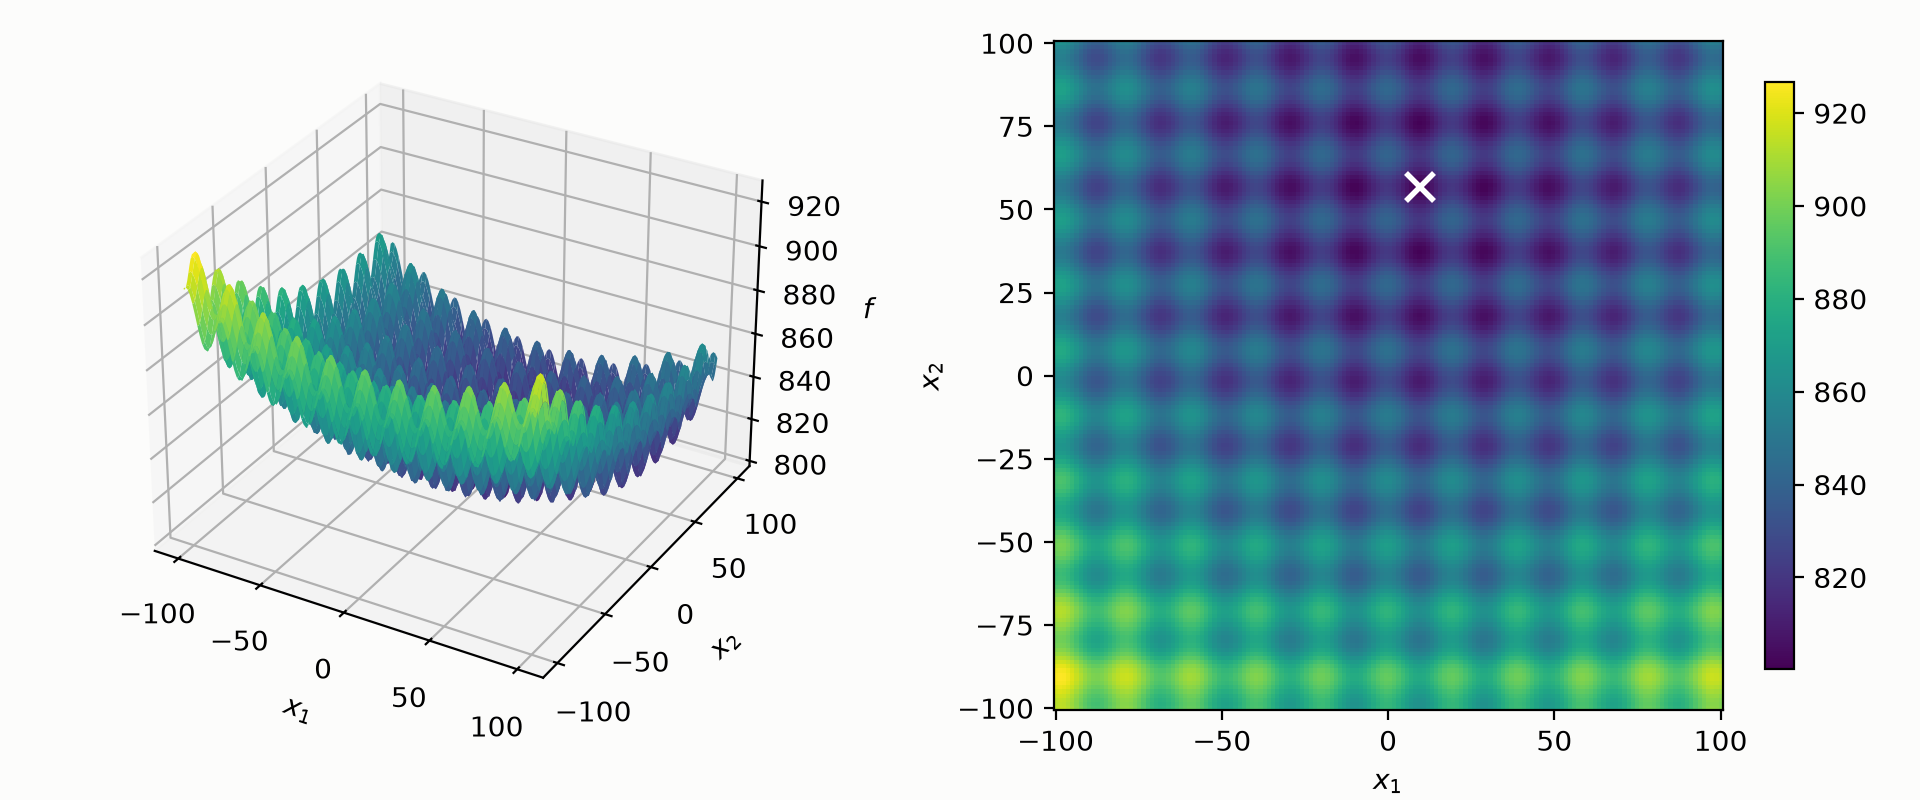
\includegraphics[width=0.92\textwidth]{function_cec2014_f8.png}
  \caption{CEC2014 F8: przekrój funkcji 10 zmiennych przez optimum w płaszczyźnie $(x_1, x_2)$.}
\end{figure}

\subsection{Wartości optimów}

Wartości optimum dla wszystkich badanych liczb zmiennych zostały odczytane z bibliotek.
Dla Ackley biblioteka zwraca $4.4\cdot10^{-16}$, czyli zero z dokładnością do błędu zaokrągleń.
Dla Schwefel stała $418.9829$ jest zaokrąglona, dlatego minimum wynosi około $1.3\cdot10^{-5}\,n$
zamiast dokładnie 0. Dla funkcji CEC punkt optimum jest wektorem przesunięcia $o$; pokazujemy jego
pierwsze trzy współrzędne (pełne wektory są w plikach danych biblioteki opfunu).

\begin{table}[H]
\centering
\small
\begin{tabular}{lrrl}
\toprule
Funkcja & $n$ & $f(x^*)$ & $x^*$ \\
\midrule
\tabinput{generated/optima.tex}
\bottomrule
\end{tabular}
\caption{Optima globalne wybranych funkcji dla 10, 20 i 30 zmiennych.}
\end{table}

\section{Eksperymenty}
\label{sec:experiments}

\subsection{Metodyka}

Konfiguracja bazowa (dla wszystkich funkcji jednakowa):
populacja 100, 1000 epok, dokładność $10^{-4}$, selekcja turniejowa (rozmiar 3),
krzyżowanie dwupunktowe ($p_k = 0.8$), mutacja jednopunktowa ($p_m = 0.2$),
inwersja ($p_i = 0.05$), elita 5\% populacji. Ułamek dla selekcji najlepszych i najgorszych
wynosi 0.3, rozmiar ziarna w krzyżowaniu ziarnistym 8 bitów.

W każdym wariancie zmieniamy względem konfiguracji bazowej tylko jeden element (metodę selekcji,
krzyżowania, mutacji albo wyłączamy elitę), dzięki czemu widać wpływ tego elementu na wynik.
Każda konfiguracja została uruchomiona 10 razy z różnymi ziarnami generatora liczb losowych.
W tabelach podajemy średni, najlepszy i najgorszy wynik z 10 uruchomień, odchylenie standardowe
oraz średni czas jednego uruchomienia. Pogrubiono najlepszą średnią. Wszystkie 480 uruchomień
wykonano kolejno w jednym procesie na tym samym komputerze (MacBook z procesorem Apple Silicon),
dzięki czemu zmierzone czasy można bezpośrednio porównywać. Wyniki pojedynczych uruchomień
(wynik i czas) są w bazie \texttt{report/data/experiments.db}.

Wykresy wartości funkcji celu oraz średniej i odchylenia standardowego w kolejnych epokach
zamieszczamy tylko dla najlepszego uruchomienia danej funkcji, czyli uruchomienia z najmniejszym
wynikiem spośród wszystkich 100 uruchomień przy 10 zmiennych (10 konfiguracji po 10 powtórzeń).

\subsection{Ackley, 10 zmiennych}
\begin{table}[H]
\centering
\small
\begin{tabular}{lrrrrr}
\toprule
\cfgtablehead
\midrule
\tabinput{generated/configs_ackley.tex}
\bottomrule
\end{tabular}
\caption{Ackley, 10 zmiennych, 10 uruchomień każdej konfiguracji ($f^* = 0$).}
\end{table}

Prawie wszystkie konfiguracje we wszystkich uruchomieniach osiągają ten sam wynik
$1.251\cdot10^{-4}$. Jest to granica wynikająca z dokładności reprezentacji. Przy dokładności
$10^{-4}$ siatka punktów na przedziale funkcji Ackley nie zawiera dokładnie zera, a najbliższy
punkt to około $\pm 3.1\cdot10^{-5}$. Mniejszy błąd można uzyskać, zwiększając dokładność.

\begin{figure}[H]
  \centering
  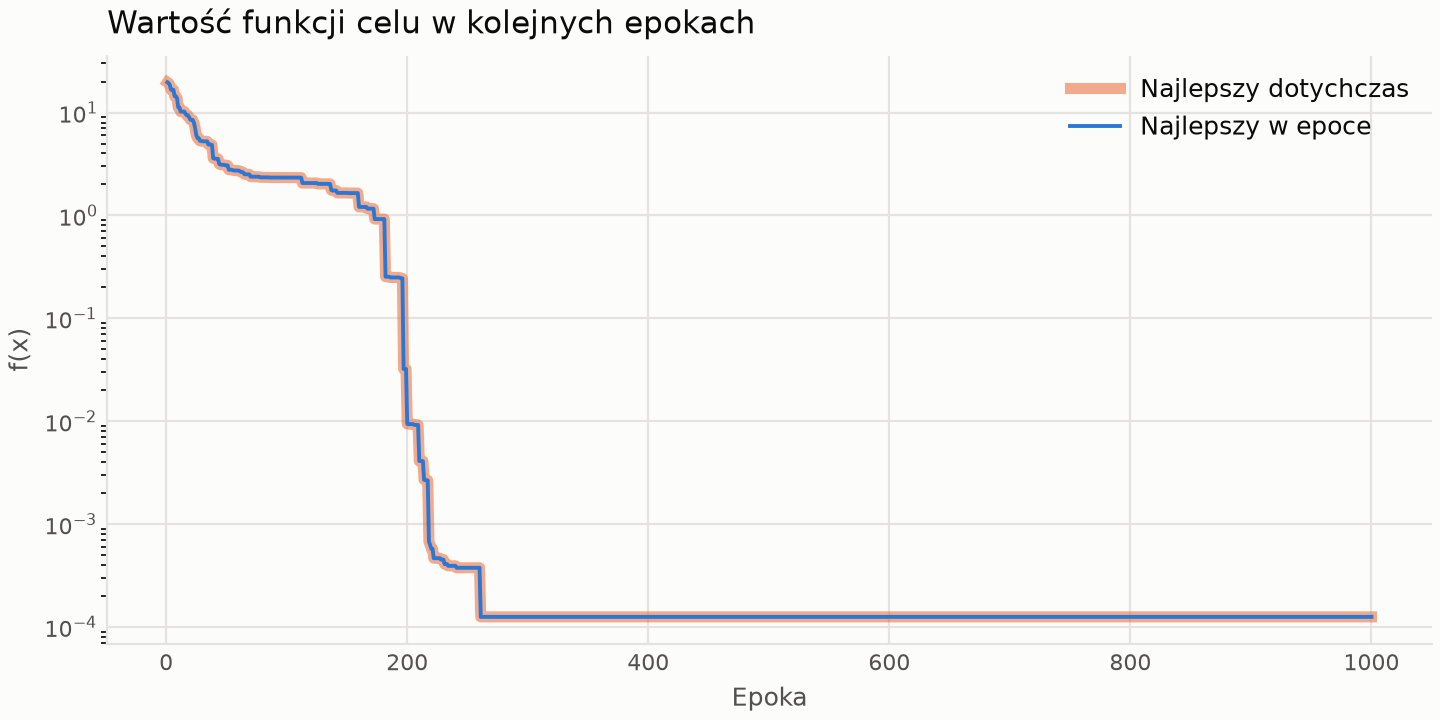
\includegraphics[width=0.8\textwidth]{best_ackley_value.png}
  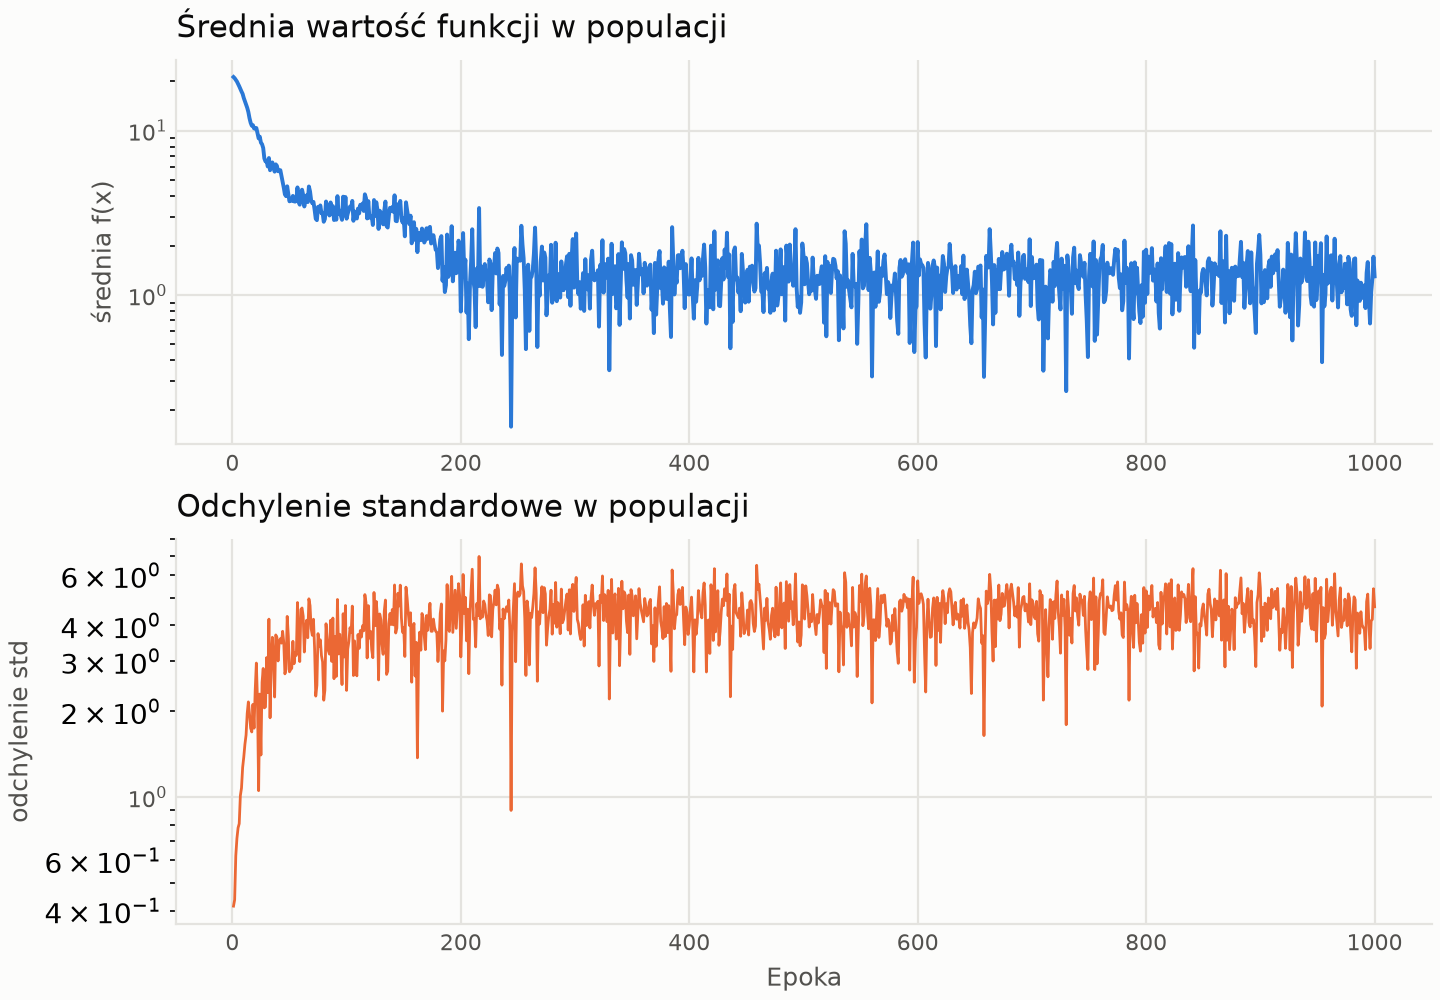
\includegraphics[width=0.8\textwidth]{best_ackley_stats.png}
  \caption{Ackley, najlepsze uruchomienie (\bestAckley). Wartość funkcji, średnia i odchylenie standardowe w kolejnych epokach (skala logarytmiczna).}
\end{figure}

\subsection{Schwefel, 10 zmiennych}
\begin{table}[H]
\centering
\small
\begin{tabular}{lrrrrr}
\toprule
\cfgtablehead
\midrule
\tabinput{generated/configs_schwefel.tex}
\bottomrule
\end{tabular}
\caption{Schwefel, 10 zmiennych ($f^* \approx 1.3\cdot10^{-4}$).}
\end{table}

\begin{figure}[H]
  \centering
  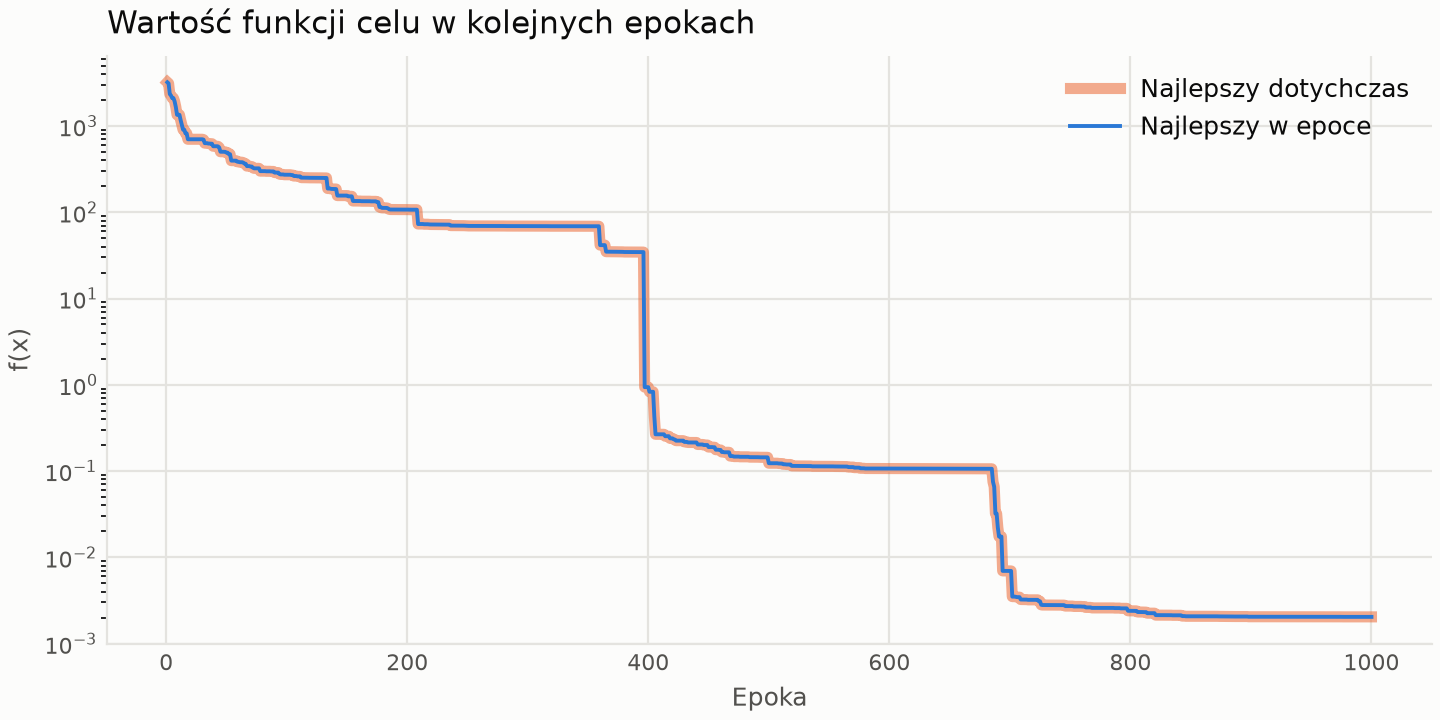
\includegraphics[width=0.8\textwidth]{best_schwefel_value.png}
  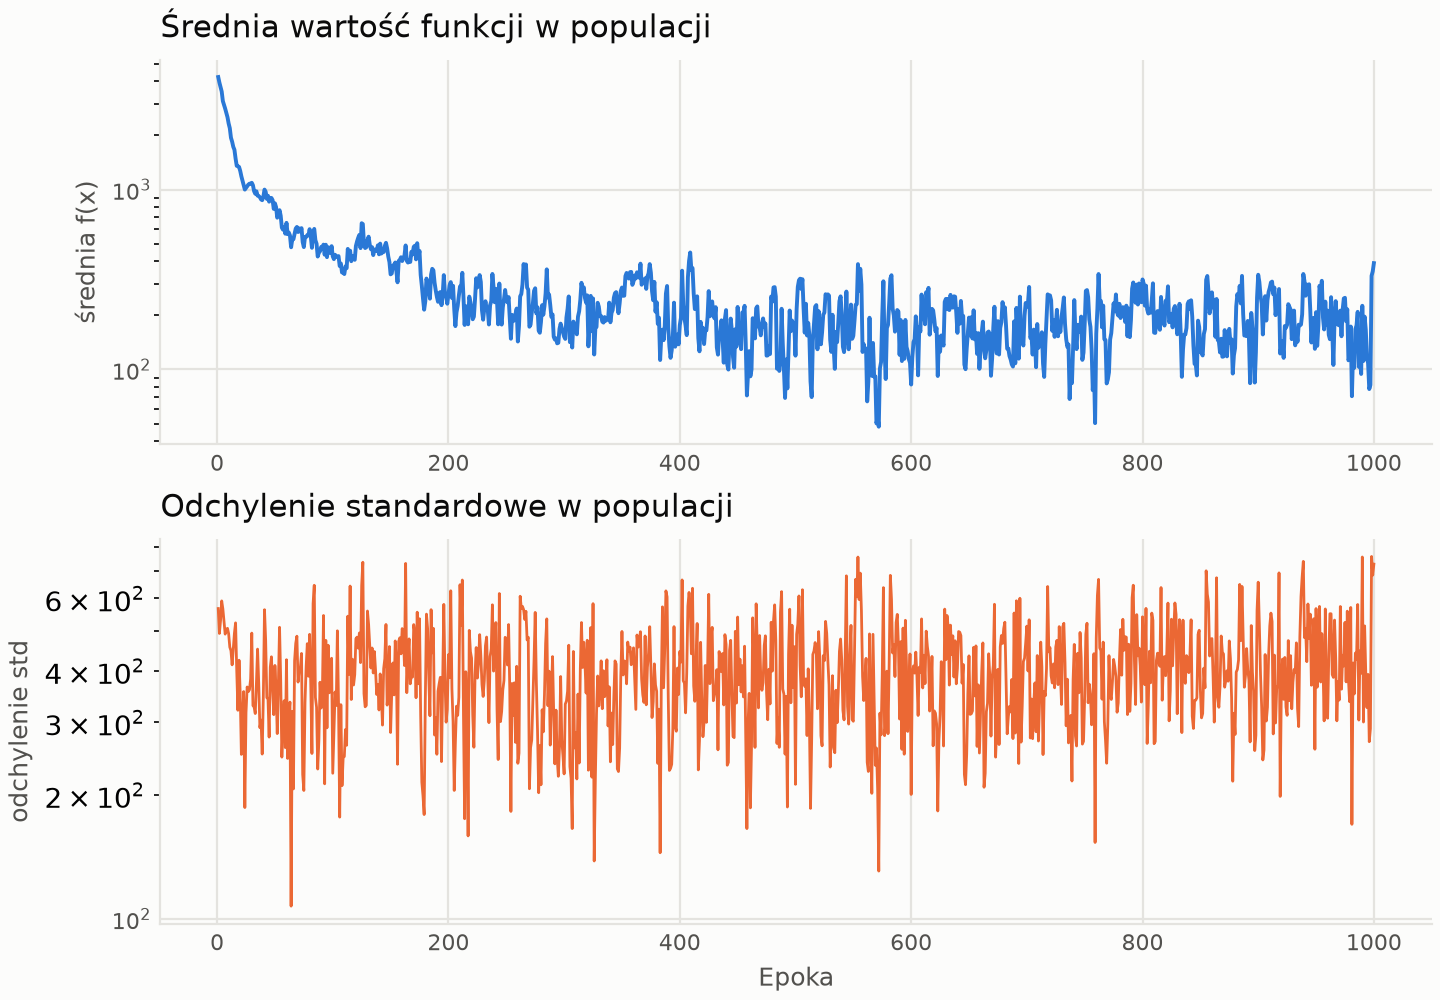
\includegraphics[width=0.8\textwidth]{best_schwefel_stats.png}
  \caption{Schwefel, najlepsze uruchomienie (\bestSchwefel).}
\end{figure}

\subsection{CEC2014 F4, 10 zmiennych}
\begin{table}[H]
\centering
\small
\begin{tabular}{lrrrrr}
\toprule
\cfgtablehead
\midrule
\tabinput{generated/configs_cec2014_f4.tex}
\bottomrule
\end{tabular}
\caption{CEC2014 F4, 10 zmiennych ($f^* = 400$).}
\end{table}

\begin{figure}[H]
  \centering
  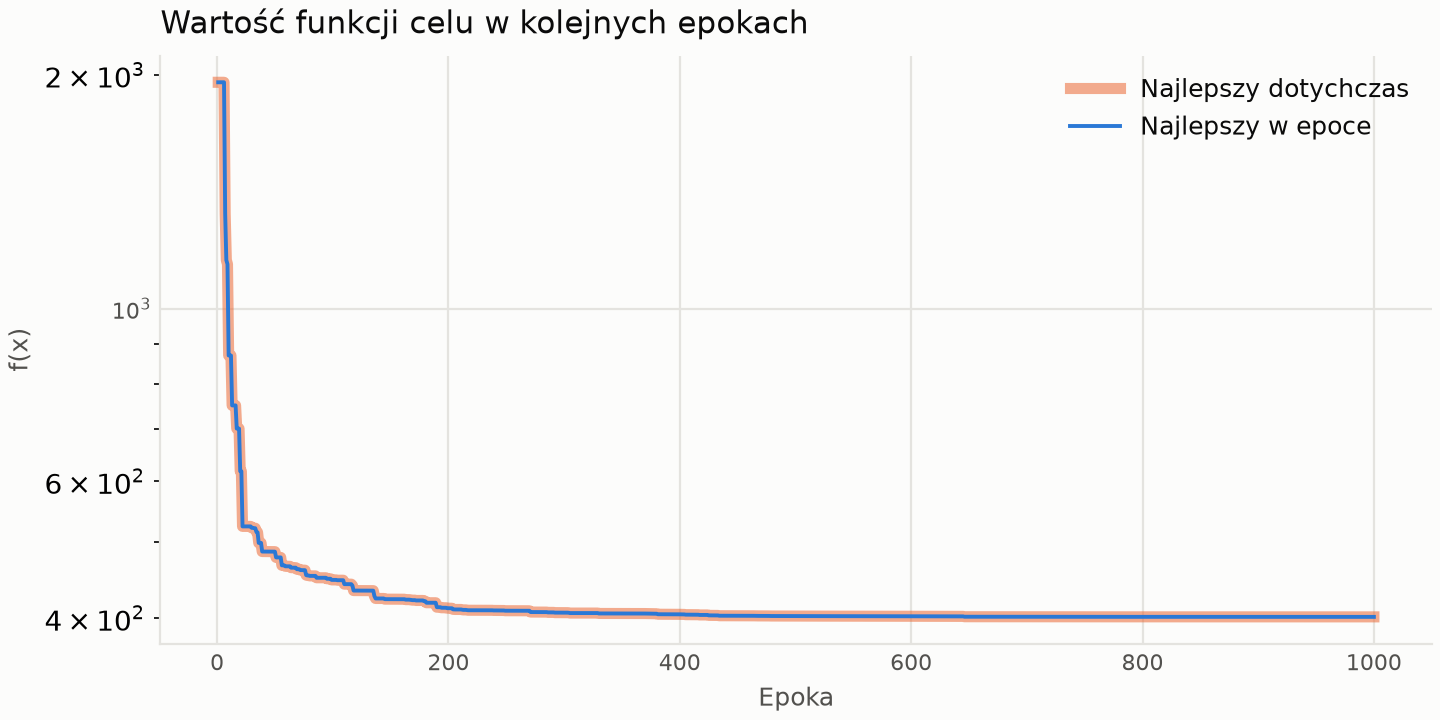
\includegraphics[width=0.8\textwidth]{best_cec2014_f4_value.png}
  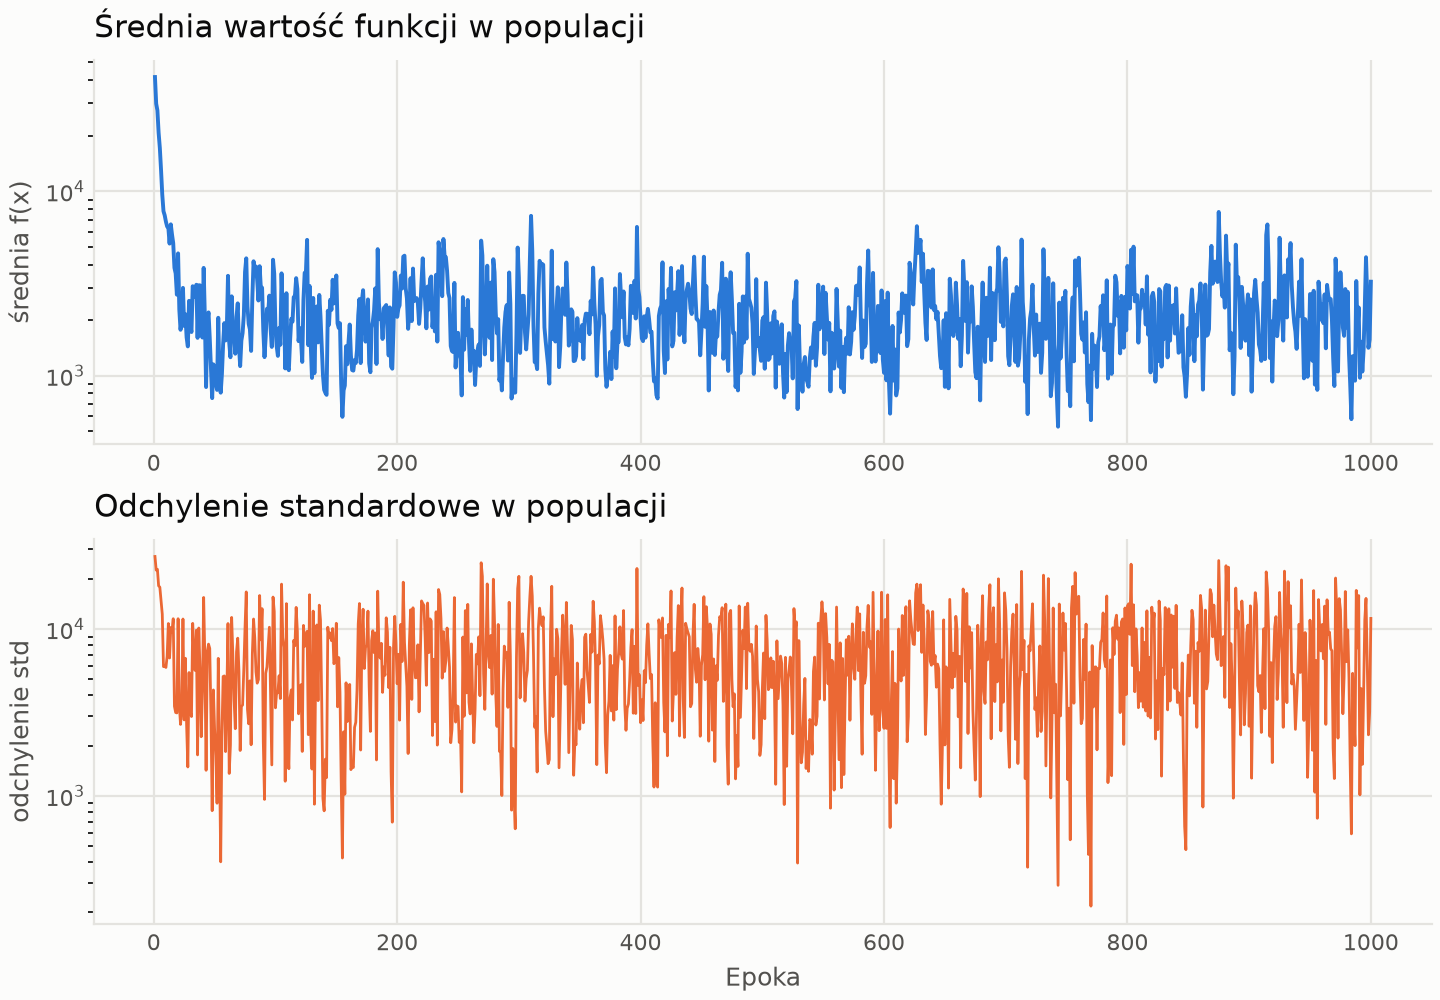
\includegraphics[width=0.8\textwidth]{best_cec2014_f4_stats.png}
  \caption{CEC2014 F4, najlepsze uruchomienie (\bestCecFour).}
\end{figure}

\subsection{CEC2014 F8, 10 zmiennych}
\begin{table}[H]
\centering
\small
\begin{tabular}{lrrrrr}
\toprule
\cfgtablehead
\midrule
\tabinput{generated/configs_cec2014_f8.tex}
\bottomrule
\end{tabular}
\caption{CEC2014 F8, 10 zmiennych ($f^* = 800$).}
\end{table}

\begin{figure}[H]
  \centering
  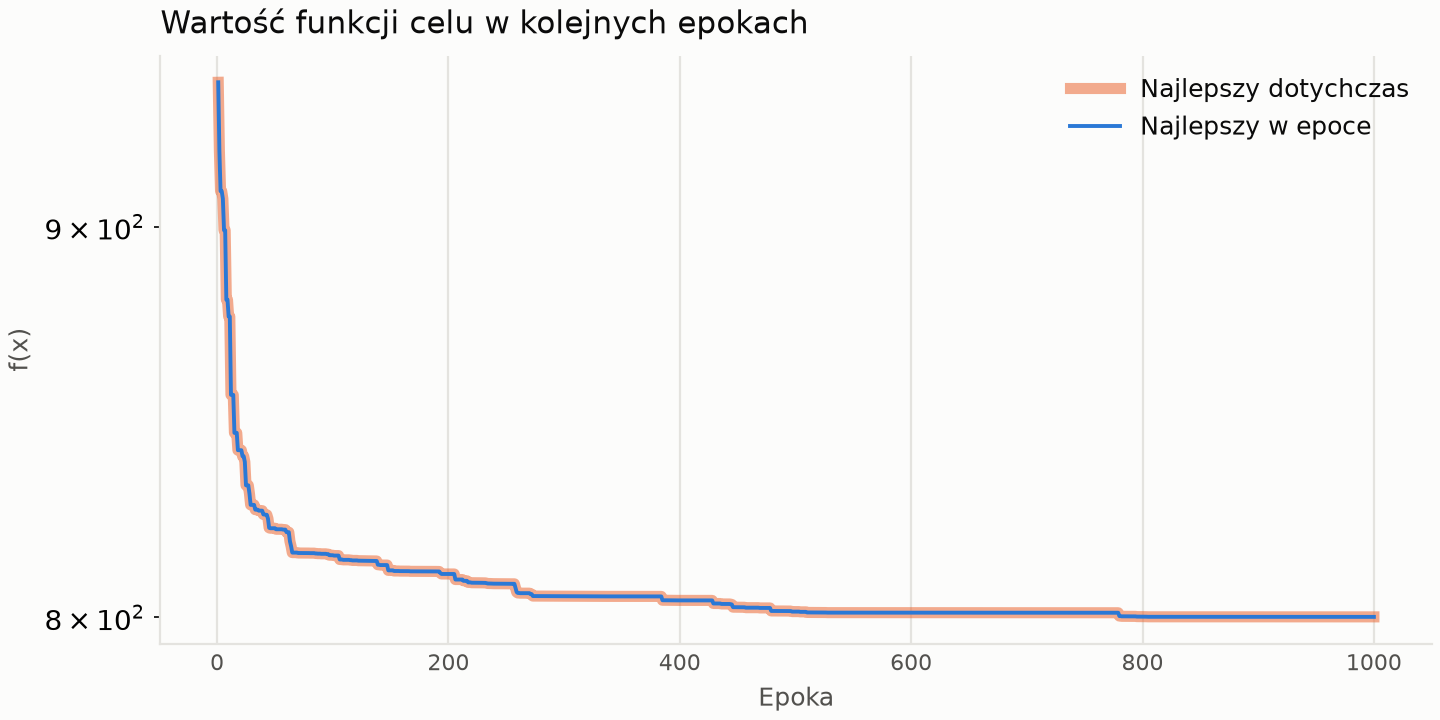
\includegraphics[width=0.8\textwidth]{best_cec2014_f8_value.png}
  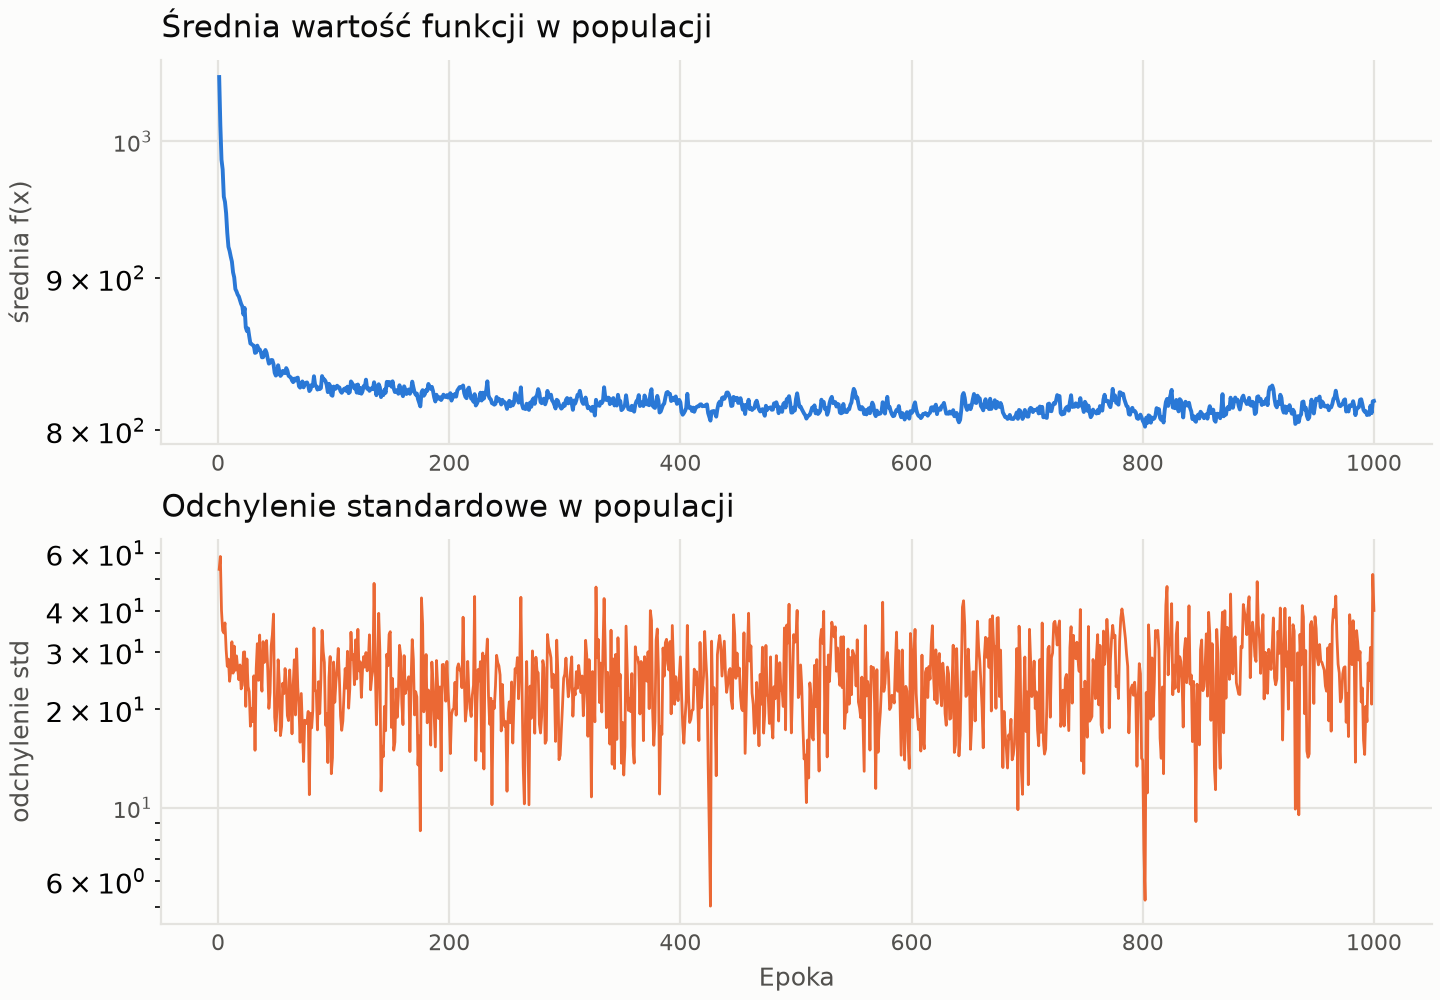
\includegraphics[width=0.8\textwidth]{best_cec2014_f8_stats.png}
  \caption{CEC2014 F8, najlepsze uruchomienie (\bestCecEight).}
\end{figure}

\subsection{Porównanie konfiguracji}

\begin{figure}[H]
  \centering
  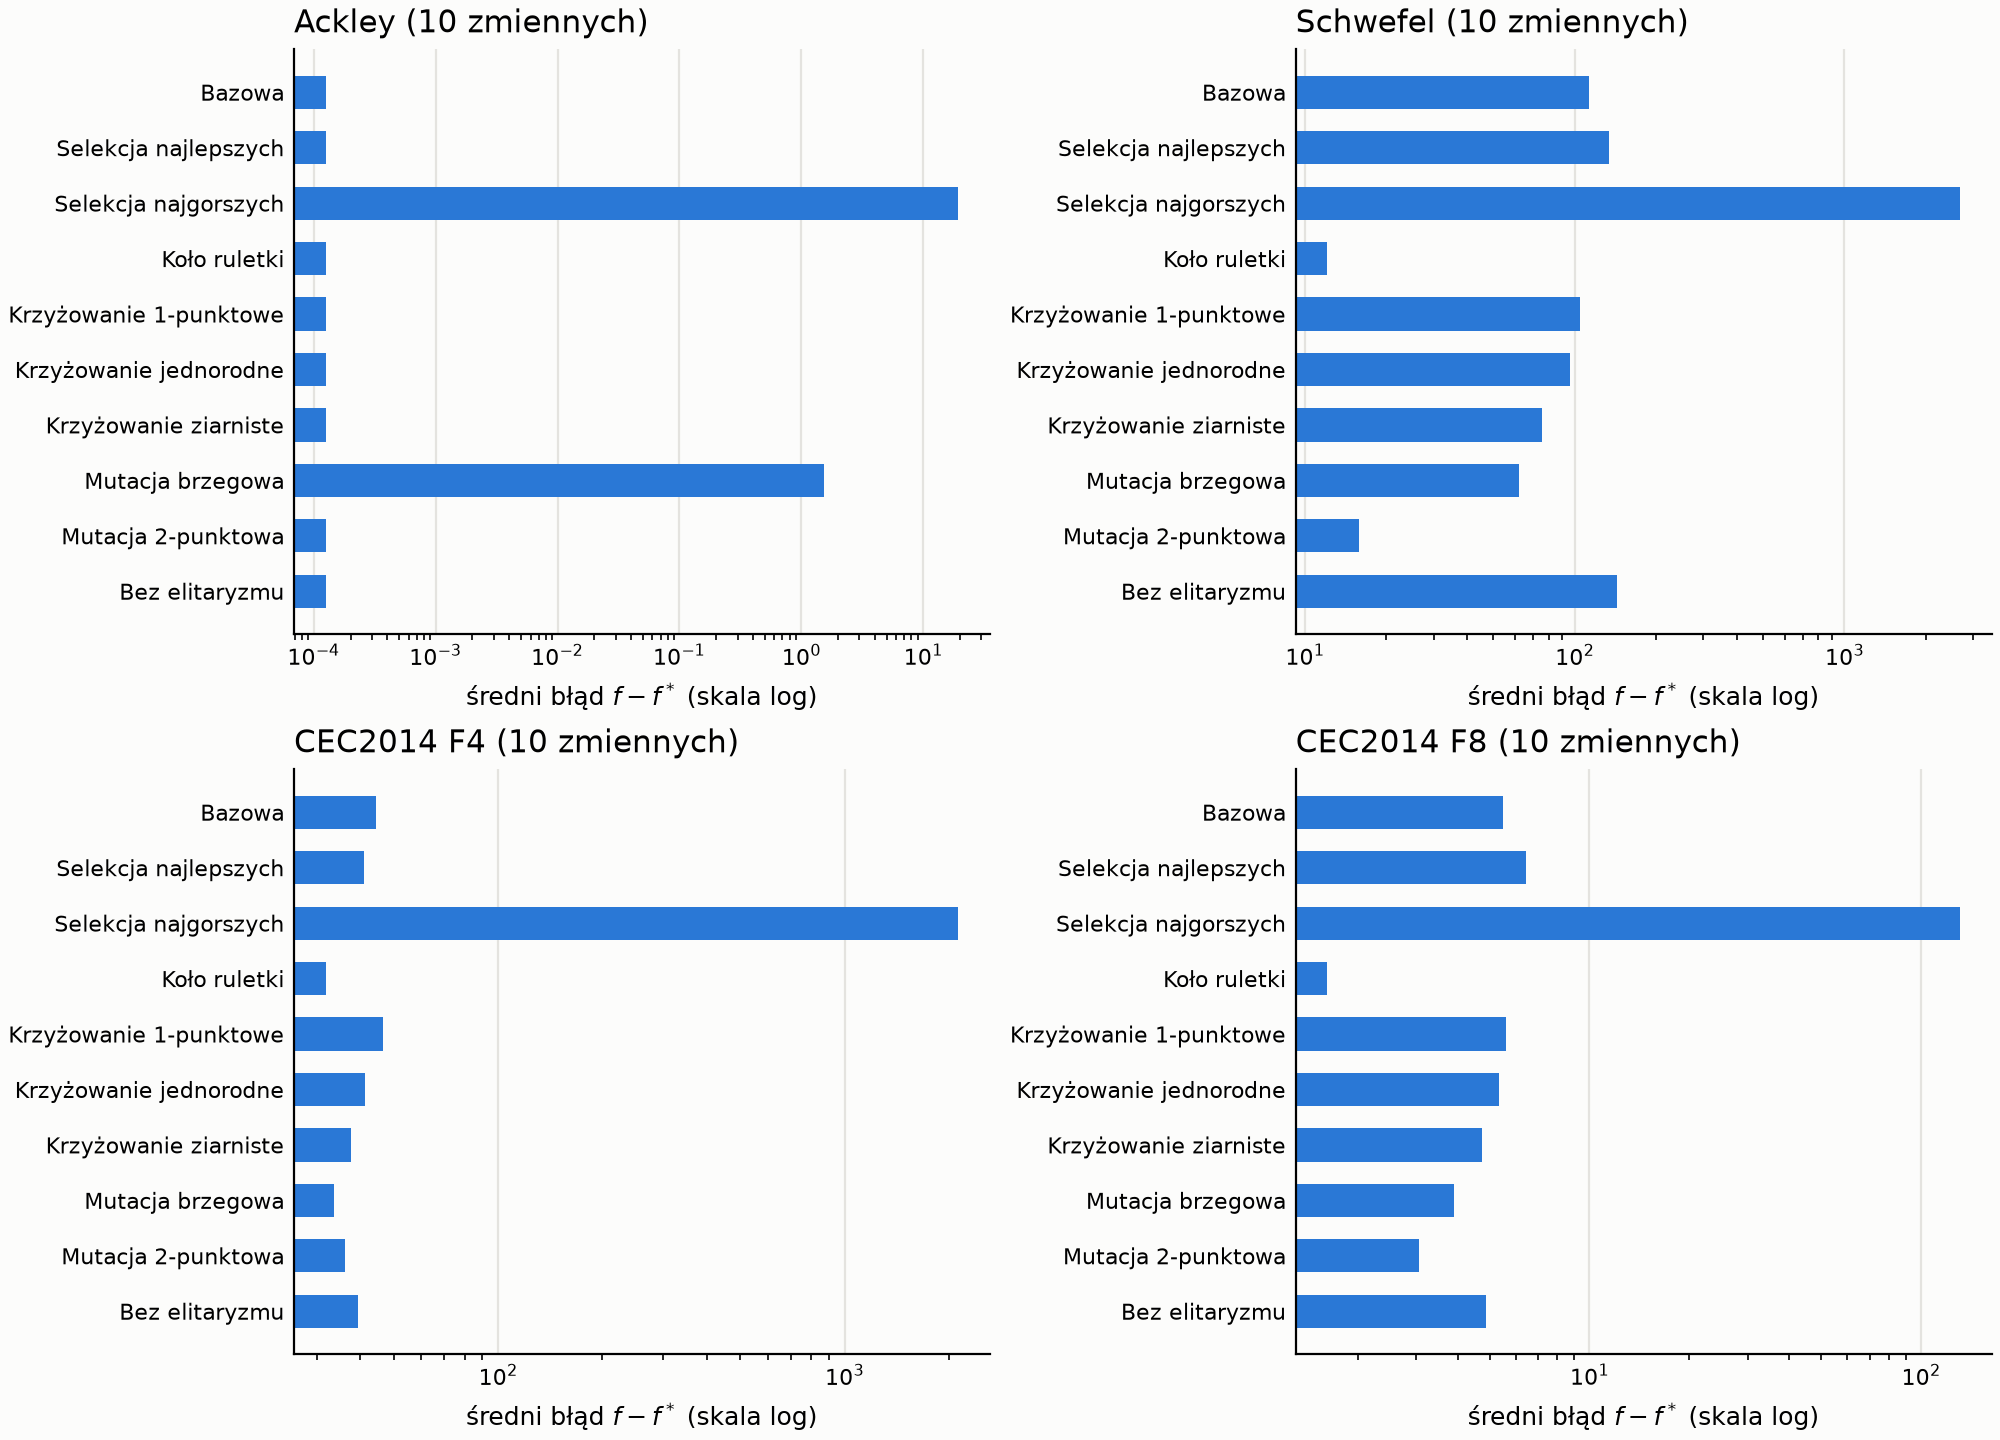
\includegraphics[width=\textwidth]{config_comparison.png}
  \caption{Średni błąd $f - f^*$ z 10 uruchomień dla każdej konfiguracji (skala logarytmiczna, mniej znaczy lepiej).}
\end{figure}

\subsection{Porównanie czasu obliczeń}

Czasy w tabelach to średni czas jednego uruchomienia (1000 epok, populacja 100). Przy 10 zmiennych
jedno uruchomienie trwa od 0.54 do 0.91 s. Najwięcej zależy od metody krzyżowania: krzyżowanie
jednopunktowe, jednorodne i ziarniste jest o około 15 do 20\% szybsze od dwupunktowego
(np. Schwefel: 0.54 s zamiast 0.67 s). Mutacja dwupunktowa jest nieco wolniejsza od jednopunktowej
(0.72 s zamiast 0.67 s), a metoda selekcji i wyłączenie elity prawie nie wpływają na czas.
Funkcje CEC liczą się dłużej niż Ackley i Schwefel (0.77 do 0.85 s w konfiguracji bazowej
zamiast 0.67 do 0.71 s), bo każde wywołanie funkcji wykonuje przesunięcie i obrót punktu.

\subsection{Wpływ liczby zmiennych}

Konfigurację bazową uruchomiliśmy również dla 20 i 30 zmiennych (po 10 razy).

\begin{table}[H]
\centering
\small
\begin{tabular}{lrrrrr}
\toprule
Funkcja & $n$ & Średnia & Najlepszy & Najgorszy & Czas [s] \\
\midrule
\tabinput{generated/dimensions.tex}
\bottomrule
\end{tabular}
\caption{Konfiguracja bazowa dla 10, 20 i 30 zmiennych.}
\end{table}

\section{Wnioski}

\begin{itemize}
  \item Funkcja Ackley jest dla algorytmu łatwa: przy 10 zmiennych wszystkie rozsądne konfiguracje
        trafiają w optimum z dokładnością ograniczoną tylko przez rozdzielczość kodowania binarnego.
        Przy 30 zmiennych chromosom ma 600 bitów i 1000 epok to za mało, by zawsze wyjść z minimów lokalnych.
  \item Selekcja najgorszych wypada najsłabiej na wszystkich funkcjach: rodzicami zostają wyłącznie
        słabe osobniki, więc postęp zapewnia praktycznie tylko elita. Mutacja brzegowa zmienia tylko
        pierwszy lub ostatni bit chromosomu, więc przy funkcji Ackley zbyt słabo eksploruje przestrzeń.
  \item Na funkcjach wielomodalnych (Schwefel, F4, F8) najlepsze średnie daje koło ruletki. Wywiera
        ono mniejszą presję selekcyjną niż turniej i dłużej utrzymuje różnorodność populacji, co
        widać na Schwefelu: średni błąd spada z około 113 do około 12.
  \item Silniejsza mutacja (dwupunktowa) wyraźnie pomaga na funkcji Schwefel i F8, ponieważ
        ułatwia przeskakiwanie między minimami lokalnymi.
  \item Rodzaj krzyżowania ma mniejszy wpływ na wynik niż selekcja i mutacja. Krzyżowanie
        jednopunktowe jest najszybsze, ziarniste daje nieco lepsze średnie na funkcjach wielomodalnych.
  \item Wyłączenie elitaryzmu wyraźnie pogorszyło wyniki na funkcji Schwefel (średnia 143.7 zamiast 113.4,
        najlepszy wynik 27.2 zamiast 0.31), bo najlepsze rozwiązanie może zostać utracone. Na funkcjach
        F4 i F8 różnica mieści się w rozrzucie wynikającym z losowości.
  \item Wraz ze wzrostem liczby zmiennych błąd szybko rośnie, a czas obliczeń rośnie wolniej
        (głównie przez dłuższe chromosomy). Dla funkcji CEC przy 20 i 30 zmiennych algorytm
        nie znajduje optimum przy tej samej liczbie epok i wielkości populacji.
  \item Funkcje CEC są trudniejsze: na F4 najlepszy wynik to $401.05$ (błąd $1.05$), na F8 $800.06$
        (błąd $0.06$), jednak średnie z 10 uruchomień są wyraźnie gorsze, co pokazuje dużą rolę losowości.
\end{itemize}

\section{Podsumowanie}

W tabeli zestawiono najlepszy wynik spośród wszystkich uruchomień dla danej funkcji i liczby
zmiennych. Błąd to różnica między osiągniętą a rzeczywistą wartością optimum.

\begin{table}[H]
\centering
\small
\begin{tabular}{lrrrrl}
\toprule
Funkcja & $n$ & Optimum $f^*$ & Wynik AG & Błąd & Konfiguracja \\
\midrule
\tabinput{generated/summary.tex}
\bottomrule
\end{tabular}
\caption{Podsumowanie: rzeczywiste optimum, najlepszy wynik algorytmu genetycznego i błąd.}
\end{table}

Nagranie przedstawiające działanie aplikacji zostało dołączone
do archiwum z projektem.

\end{document}
